%%%%%%%%%%%%%%%%%%%%%%%%%%%%%%%%%%%%%%%%%%%%%%%%%%%%%%%%%%%%%%%%%
%%% %
%%% % weiiszablon.tex
%%% % The Faculty of Electrical and Computer Engineering
%%% % Rzeszow University Of Technology diploma thesis Template
%%% % Szablon pracy dyplomowej Wydziału Elektrotechniki 
%%% % i Informatyki PRz
%%% % June, 2015
%%%%%%%%%%%%%%%%%%%%%%%%%%%%%%%%%%%%%%%%%%%%%%%%%%%%%%%%%%%%%%%%%
\documentclass[12pt]{article}

\usepackage{weiiszablon}

\author{Jakub Kusal}

% np. EF-123456, EN-654321, ...
\studentID{EF-169571}

\title{HuePi - aplikacja mobilna do obsługi żarówek Philips Hue}
\titleEN{HuePi - mobile app for managing Philips Hue bulbs}


%%% wybierz rodzaj pracy wpisując jeden z poniższych numerów: ...
% 1 = inżynierska	% BSc
% 2 = magisterska	% MSc
% 3 = doktorska		% PhD
%%% na miejsce zera w linijce poniżej
\newcommand{\rodzajPracyNo}{1}


%%% promotor
\supervisor{dr inż. Mariusz Mączka}
%% przykład: dr hab. inż. Józef Nowak, prof. PRz

%%% promotor ze stopniami naukowymi po angielsku
\supervisorEN{Mariusz Mączka, BEng, PhD}

\abstract{Projekt HuePi to aplikacja mobilna umożliwiająca sterowanie oświetleniem Philips Hue przez serwer na Raspberry Pi. Wykorzystuje nowoczesne technologie, takie jak
FastAPI, Retrofit i Jetpack Compose. Umożliwia zarządzanie światłami, regulację jasności, zmianę kolorów oraz dynamiczne dostosowanie barwy do temperatury otoczenia.}
\abstractEN{The HuePi project is a mobile app for controlling Philips Hue lighting via a Raspberry Pi server. It employs modern technologies such as FastAPI, Retrofit, and Jetpack Compose.
The app enables light management, brightness control, color adjustments, and dynamic color adaptation based on ambient temperature.}

\begin{document}

% strona tytułowa
\maketitle

\blankpage

% spis treści
\tableofcontents

\clearpage
\blankpage


\section{Wstęp}
Używanie urządzeń typu \textit{Smart Home} cieszy się dziś coraz większym zainteresowaniem. \cite{popularność-smart-home} Nie jest to już
tylko ciekawostka technologiczna, która musi wiązać się z dużymi wydatkami.
Urządzenia tego typu stają się coraz bardziej przystępne cenowo, a producenci oferują coraz to większy wybór
samych urządzeń końcowych, jak i urządzeń integrujących całą resztę. Do takich urządzeń możemy zaliczyć m.in.:
kamery, zamki, głośniki, wyświetlacze, termostaty, gniazdka, żarówki itp. Widać więc, że spośród całej gamy urządzeń, mamy do wyboru opcje takie,
które pomagają zautomatyzować i wspomóc życie ludzi, jak również takie, które służą rozrywce.\\
Tym ostatnim typem urządzeń zajęto się w tym projekcie. Jego celem było stworzenie aplikacji mobilnej Android,
umożliwiającej sterowanie żarówkami producenta Philips, z serii Philips Hue.
Jest to cały ekosystem smart urządzeń, nie tylko żarówek. W jego skład wchodzą m.in. również:
paski LED, lampy stojące, lampki "choinkowe", przyciski, gniazdka, kamery, czujniki ruchu, czujniki zmierzchu.\\
Mimo ogromnej gamy urządzeń, można jednak zauważyć, iż nie występują w tym systemie żadnego rodzaju czujniki temperatury, czy sensory innych warunków atmosferycznych.
Tego typu akcesorium, mogłoby rozszerzyć, już jakże szeroki wachlarz możliwości ekosystemu Philips Hue, dzięki któremu korzystanie z np. żarówek stałoby się jeszcze bardziej ekscytujące.
Niniejszy projekt celuje w wypełnienie luki powstałej z faktu braku występowania wyżej wymienionych sensorów i przedstawienie konceptu, który pokazuje,
jak natywny ekosystem Philips Hue mógłby się rozwinąć.


\clearpage

\section{Cel oraz zakres projektu}
Celem projektu, było stworzenie aplikacji mobilnej na systemy operacyjne Android, przeznaczonej do sterowania żarówkami Philips Hue.
Nie stanowi ona pełnoprawnego oprogramowania do sterowania każdym produktem z ekosystemu Philips Hue.
Poza podstawowymi funkcjonalnościami, ma ona ukazać możliwości, o jakie możnaby rozszerzyć natywne ekosystemy Philips Hue.
Oprócz klasycznego sterowania, tj. ustawienie koloru, jasności, włączenia i wyłączenia, aplikacja miała umożliwiać wykorzystanie informacji o temperaturze,
w celu wyświetlania kolorów na podstawie tejże temperatury.


\subsection{Podobne oprogramowanie}
Pomysł na tego typu aplikację nie jest nowy. Istnieje wiele systemów, aplikacji i oprogramowania, które implementują funkcjonalności w zaprezentowanej tutaj aplikacji
i mają podobną filozofię. Przykłady niektórych z nich to:

\subsubsection{Philips Hue (aplikacja producenta)}
Philips Hue to oficjalna aplikacja mobilna producenta, przeznaczona głównie do zarządzania inteligentnym oświetleniem z rodziny Hue.
Udostępniana jest na urządzenia z systemem \textit{Android} oraz \textit{iOS},a jej podstawowym zadaniem jest umożliwienie pełnej konfiguracji i kontroli wszystkich elementów tego ekosystemu,
włącznie z tworzeniem scen, harmonogramów oraz automatyzacji.\\
Aplikacja komunikuje się z mostkiem Philips Hue, który jest fizycznym urządzeniem pełniącym rolę pośrednika pomiędzy oświetleniem a siecią lokalną.
Bezpośrednia integracja z mostkiem umożliwia:
\begin{itemize} \item dodawanie nowych żarówek lub innych akcesoriów (np. czujników ruchu, gniazdek) do ekosystemu,
    \item tworzenie i edytowanie tzw. \textit{scen świetlnych} (zestawów preferowanych ustawień światła, takich jak kolor, jasność czy temperatura barwowa),
    \item planowanie harmonogramów, pozwalających automatycznie włączać lub wyłączać światło o wybranych porach dnia,
    \item sterowanie głosowe (po odpowiedniej konfiguracji z asystentami pokroju Amazon Alexa, Apple Siri czy Google Assistant),
    \item konfigurowanie prostych reguł automatyzacji, które mogą reagować np. na wykrycie ruchu.
\end{itemize}
Korzystanie z aplikacji Philips Hue pozwala w łatwy sposób zapanować nad całym ekosystemem oświetlenia inteligentnego,
jednakże nie wspiera ona pomiaru parametrów środowiskowych, takich jak temperatura czy wilgotność.
W efekcie, choć zaspokaja większość typowych potrzeb związanych z inteligentnym oświetleniem,
nie rozszerza funkcjonalności systemu o dodatkowe odczyty czy też automatyzacje bazujące na czynnikach zewnętrznych (m.in. z użyciem czujników temperatury). \cite{dokumentacja-philips-hue-app}

\subsubsection{Home Assistant}
Home Assistant to otwartoźródłowe oprogramowanie przeznaczone do lokalnego zarządzania i automatyzacji urządzeń w inteligentnym domu.
Można je wdrożyć zarówno na komputerach jednopłytkowych (np. Raspberry Pi), jak i na serwerach czy w środowisku kontenerowym (np. Docker).
Dzięki temu jest rozwiązaniem elastycznym pod względem wymagań sprzętowych i sposobu instalacji.\\
Dużą zaletą Home Assistant jest bogaty ekosystem integracji, który obejmuje również wsparcie
dla oświetlenia Philips Hue. Oprócz podstawowego sterowania, możliwe jest konfigurowanie zaawansowanych reguł automatyzacji,
reagujących np. na informacje z rozmaitych czujników (temperatury, wilgotności czy ruchu).
Platforma oferuje wbudowany edytor scen i skryptów, pozwalający na tworzenie wieloetapowych akcji wyzwalanych przez określone zdarzenia
(bądź harmonogramy czasowe).\\
Home Assistant zapewnia także dostęp do panelu webowego, dzięki któremu w wygodny sposób można zarządzać urządzeniami,
przeglądać ich status, a także dostosowywać interfejs użytkownika zgodnie z własnymi preferencjami.
Ze względu na swoją otwartość i rozbudowaną społeczność, umożliwia wprowadzanie dodatkowych wtyczek (\textit{add-ons})
i komponentów, co sprawia, że możliwości systemu są praktycznie nieograniczone.
Duża liczba gotowych rozwiązań udostępnianych w formie repozytoriów społecznościowych pozwala
szybko uruchamiać nowe funkcjonalności lub modyfikować istniejące. \cite{dokumentacja-home-assistant}

\subsubsection{Google Home}
Google Home to platforma i aplikacja mobilna rozwijana przez firmę Google, służąca do zarządzania urządzeniami inteligentnego domu.
W odróżnieniu od rozwiązań stricte samodzielnych, aplikacja ta ściśle integruje się z ekosystemem usług Google oraz asystentem głosowym Google Assistant,
co pozwala sterować wieloma sprzętami za pomocą komend głosowych.\\
Podobnie jak inne rozwiązania z tej kategorii, Google Home obsługuje oświetlenie Philips Hue, umożliwiając jego konfigurację, tworzenie tzw. pokoi (ang. \textit{rooms})
i grupowanie urządzeń w praktyczny sposób. Pozwala także w prosty sposób zaprogramować podstawowe sceny świetlne czy harmonogramy włączania i wyłączania.
Ze względu na powiązania z kontem Google, cała konfiguracja pozostaje dostępna z różnych urządzeń (smartfon, tablet, głośniki Nest itp.),
co ułatwia zdalne sterowanie oświetleniem oraz innymi elementami inteligentnego domu (np. termostatami, głośnikami czy kamerami).\\
W przeciwieństwie do bardziej zaawansowanych platform otwartoźródłowych, Google Home koncentruje się głównie na wygodzie i prostocie użytkowania.
Oferuje co prawda możliwość definiowania automatyzacji – tzw. \textit{Routines} – jednak nie pozwala na tak rozbudowane scenariusze integracji,
jak systemy pokroju Home Assistant. Niemniej jednak dzięki swojemu podejściu „wszystko w jednym” i ścisłemu powiązaniu z usługami Google,
Google Home jest dobrym wyborem dla użytkowników szukających łatwego w konfiguracji i intuicyjnego rozwiązania do codziennego sterowania oświetleniem Philips Hue,
jak również innymi urządzeniami typu \textit{Smart Home}. \cite{dokumentacja-google-home}

\clearpage

\section{Wykorzystany sprzęt i technologie}
Projekt można podzielić na 2 główne części: serwer uruchomiony na Raspberry Pi 3B wraz z czujnikiem oraz aplikacja moblina.
\subsection{Serwer na Raspberry Pi}

\subsubsection{Raspberry Pi 3B}
Raspberry Pi 3B to komputer jednopłytkowy opracowany przez fundację Raspberry Pi, który od momentu wprowadzenia na rynek zdobył ogromną popularność zarówno wśród hobbystów,
jak i profesjonalistów. Jego niewielkie wymiary (85.6 mm x 56.5 mm) oraz niska cena sprawiają,
że stanowi doskonałe rozwiązanie do tworzenia różnorodnych projektów technologicznych, takich jak systemy \textit{Smart Home},
urządzenia IoT (Internet of Things), serwery multimedialne, a nawet jako komputer edukacyjny.
Raspberry Pi 3B jest wyposażony w czterordzeniowy procesor ARM Cortex-A53 o taktowaniu 1.2 GHz, co w połączeniu z 1 GB pamięci RAM
pozwala na płynne działanie lekkich systemów operacyjnych, takich jak Raspberry Pi OS, Ubuntu czy inne dystrybucje Linuxa zoptymalizowane pod kątem architektury ARM.
Wbudowana karta Wi-Fi obsługująca standard 802.11n oraz moduł Bluetooth 4.1 umożliwiają bezprzewodową komunikację z innymi urządzeniami
oraz sieciami lokalnymi bez konieczności stosowania dodatkowych adapterów.\\
Płyta oferuje liczne interfejsy wejścia i wyjścia, co czyni ją wyjątkowo wszechstronną w zastosowaniach praktycznych. Na wyposażeniu znajdują się m.in.:
\begin{itemize}
    \item 40-pinowy złącze GPIO (\textit{General Purpose Input/Output}), które umożliwia podłączanie i sterowanie szeroką gamą urządzeń peryferyjnych,
          takich jak czujniki, diody LED, przyciski czy serwomechanizmy,
    \item 4 porty USB 2.0, umożliwiające podłączenie akcesoriów takich jak klawiatura, mysz, kamera czy pendrive,
    \item złącze HDMI do podłączenia monitora, co pozwala na wykorzystanie urządzenia jako miniaturowego komputera stacjonarnego,
    \item złącze CSI do kamer i DSI do ekranów, co otwiera możliwości budowy systemów monitoringu czy interaktywnych wyświetlaczy,
    \item interfejsy komunikacyjne, takie jak \textit{I\textsuperscript{2}C}, \textit{SPI} i \textit{UART}, służące do komunikacji z różnymi modułami i sensorami.
\end{itemize}
Jednym z przykładów modułów, które mogą być zintegrowane z Raspberry Pi 3B, jest czujnik BME280. Urządzenie to umożliwia precyzyjne pomiary temperatury,
wilgotności oraz ciśnienia atmosferycznego. Dzięki swoim kompaktowym wymiarom i wsparciu dla interfejsu \textit{I\textsuperscript{2}C},
czujnik BME280 jest często wykorzystywany w projektach związanych z monitorowaniem warunków środowiskowych, systemami \textit{Smart Home}
czy urządzeniami prognozującymi pogodę. Raspberry Pi 3B, w połączeniu z takim czujnikiem, może odczytywać dane w czasie rzeczywistym,
co pozwala na ich dalsze przetwarzanie oraz wykorzystanie w aplikacjach automatyzacji lub raportowania. Dzięki wielu dostępnym bibliotekom,
integracja czujnika z urządzeniem jest stosunkowo prosta i szybka.\\
Raspberry Pi 3B wspiera również wiele oprogramowania pozwalającego na wygodną integrację z urządzeniami \textit{Smart Home}.
Na przykład, instalacja platform takich jak poprzednio omawiany Home Assistant umożliwia tworzenie zaawansowanych reguł automatyzacji
oraz centralne zarządzanie wieloma urządzeniami, w tym oświetleniem Philips Hue. Możliwość uruchamiania serwerów lokalnych (np. HTTP czy MQTT) sprawia,
że Raspberry Pi może pełnić rolę centrum sterowania lub bramy komunikacyjnej w bardziej rozbudowanych projektach.\\
Dzięki aktywnej społeczności użytkowników, Raspberry Pi 3B jest dobrze udokumentowany, a w sieci dostępne są liczne poradniki i przykłady implementacji projektów.
Wszechstronność i niska cena tego komputera sprawiają, że jest on chętnie wybierany zarówno do celów edukacyjnych, jak i komercyjnych.
Raspberry Pi 3B może być zatem kluczowym elementem projektów opartych na inteligentnym oświetleniu, takich jak \textit{HuePi},
w których służy jako serwer API przetwarzający dane z sensorów oraz komunikujący się z żarówkami w ekosystemie Philips Hue.


\subsubsection{Czujnik BME280}
Czujnik BME280 to wielofunkcyjny sensor środowiskowy opracowany przez firmę Bosch, przeznaczony do pomiaru trzech podstawowych parametrów:
temperatury, wilgotności oraz ciśnienia atmosferycznego. Ze względu na swoją wszechstronność, kompaktowe rozmiary oraz wysoką precyzję pomiarów,
znajduje szerokie zastosowanie w projektach związanych z automatyką domową, Internetem Rzeczy (IoT) oraz urządzeniami monitorującymi warunki środowiskowe.\\
BME280 wspiera interfejsy komunikacyjne \textit{I\textsuperscript{2}C} oraz \textit{SPI}, co czyni go łatwym do integracji z różnymi mikrokontrolerami i komputerami jednopłytkowymi,
takimi jak Raspberry Pi. Dzięki temu użytkownik ma dużą elastyczność w wyborze platformy sprzętowej. Czujnik charakteryzuje się niskim zużyciem energii,
co sprawia, że idealnie nadaje się do zastosowań w systemach zasilanych bateryjnie.\\
Specyfikacja czujnika obejmuje:
\begin{itemize}
    \item Zakres pomiaru temperatury: od -40°C do +85°C, z dokładnością do ±1°C\cite{bme280-datasheet},
    \item Zakres pomiaru wilgotności: od 0\% do 100\% RH (wilgotność względna), z dokładnością ±3\% RH\cite{bme280-datasheet},
    \item Zakres pomiaru ciśnienia atmosferycznego: od 300 hPa do 1100 hPa, z dokładnością do ±1 hPa\cite{bme280-datasheet}.
\end{itemize}
Czujnik jest wykorzystywany w aplikacjach takich jak:
\begin{itemize}
    \item monitorowanie warunków środowiskowych w budynkach (np. wilgotność w pomieszczeniach mieszkalnych),
    \item systemy pogodowe, w tym prognozowanie zmian ciśnienia,
    \item automatyzacja domowa, np. w połączeniu z systemami sterowania oświetleniem, które mogą reagować na zmiany temperatury,
    \item urządzenia IoT, zbierające dane do analizy i przesyłające je do systemów chmurowych lub lokalnych serwerów.
\end{itemize}
Czujnik BME280 jest często wykorzystywany w projektach prototypowych i edukacyjnych dzięki szerokiej dostępności bibliotek programistycznych.
Możliwość dokładnych pomiarów w połączeniu z łatwością integracji sprawia, że czujnik ten idealnie nadaje się do implementacji w projektach
takich jak \textit{HuePi}, w których dane np. o temperaturze mogą być przetwarzane w celu dostosowania funkcji systemu, np. sterowania oświetleniem.

\subsubsection{FastAPI}
FastAPI to nowoczesny framework do tworzenia aplikacji webowych oraz API w języku Python. Został zaprojektowany z myślą o wysokiej wydajności,
prostocie użytkowania oraz integracji z typowaniem statycznym w Pythonie. Dzięki zastosowaniu standardu ASGI (Asynchronous Server Gateway Interface),
FastAPI wspiera obsługę zapytań w trybie asynchronicznym, co czyni go szczególnie przydatnym w aplikacjach wymagających dużej liczby jednoczesnych zapytań
lub intensywnej komunikacji z zewnętrznymi usługami.
FastAPI jest oparty na narzędziu \textit{Starlette} (do obsługi zapytań i trasowania) oraz \textit{Pydantic} (do walidacji i serializacji danych).
Oferuje funkcjonalności, które czynią go jednym z najpopularniejszych frameworków do budowy API, takich jak:
\begin{itemize}
    \item Automatyczne generowanie dokumentacji API na podstawie definicji punktów końcowych (\textit{endpoints}) i typów danych. \cite{fastapi-automatyczna-dokumentacja}
          Dokumentacja jest dostępna w formatach \textit{Swagger UI} oraz \textit{ReDoc}, co ułatwia testowanie i integrację API.
    \item Wsparcie dla typowania w Pythonie, co umożliwia precyzyjne określenie wejściowych i wyjściowych danych dla punktów końcowych.
          Typowanie pozwala również na automatyczną walidację danych i zmniejsza ryzyko błędów programistycznych.
    \item Obsługa asynchroniczności dzięki natywnemu wsparciu dla konstrukcji \texttt{async} i \texttt{await}, co sprawia,
          że framework doskonale sprawdza się w aplikacjach wymagających współbieżności, takich jak przetwarzanie danych w czasie rzeczywistym czy obsługa mikroserwisów.
    \item Łatwa integracja z systemami autoryzacji i uwierzytelniania, np. przy użyciu protokołów OAuth2 czy JWT (\textit{JSON Web Tokens}).
    \item Rozbudowane wsparcie dla operacji związanych z przetwarzaniem żądań HTTP, takich jak pobieranie danych z parametrów,
          nagłówków czy plików przesyłanych przez użytkowników.
\end{itemize}
FastAPI znajduje zastosowanie w wielu obszarach, takich jak:
\begin{itemize}
    \item Tworzenie mikroserwisów – dzięki asynchroniczności i wysokiej wydajności framework świetnie nadaje się do budowy modułowych aplikacji o niewielkiej złożoności.
    \item Systemy IoT – FastAPI może być używane jako interfejs do komunikacji między urządzeniami a centralnym serwerem.
    \item Tworzenie RESTful API – pozwala na szybkie i efektywne tworzenie punktów końcowych dla aplikacji webowych czy mobilnych.
    \item Integracja z systemami ML/AI – FastAPI jest często wykorzystywane do udostępniania modeli uczenia maszynowego w formie usług API,
          umożliwiających ich łatwą integrację z innymi aplikacjami.
\end{itemize}
Dzięki intuicyjnej składni, bogatej dokumentacji oraz dużej społeczności użytkowników, FastAPI stał się jednym z najchętniej wybieranych narzędzi
do budowy nowoczesnych aplikacji webowych i API w Pythonie.

\subsection{Aplikacja mobilna}

\subsubsection{Język Kotlin}
Kotlin to nowoczesny, wieloplatformowy język programowania opracowany przez firmę JetBrains. Jego pierwsza stabilna wersja została wydana w 2016 roku \cite{kotlin-data-wydania},
a już w 2017 roku został oficjalnie ogłoszony przez Google jako język wspierany do tworzenia aplikacji na system Android.
Kotlin został zaprojektowany jako nowoczesna alternatywa dla Javy, oferująca większą produktywność, czytelność kodu oraz nowoczesne funkcje,
które redukują ryzyko błędów programistycznych.\\
Kotlin jest językiem zorientowanym obiektowo z elementami programowania funkcyjnego. Wyróżnia go pełna interoperacyjność z kodem napisanym w Javie,
co umożliwia łatwą migrację istniejących projektów. Dzięki temu programiści mogą stopniowo wprowadzać Kotlin do swoich aplikacji,
korzystając z bibliotek i narzędzi napisanych w Javie.\\
Jednym z kluczowych powodów popularyzacji Kotlina jest fakt, że Google wymaga jego użycia do pracy z Jetpack Compose – nowoczesnym narzędziem
do tworzenia interfejsów użytkownika w aplikacjach na system Android. Dzięki Jetpack Compose, aplikacje mogą być projektowane szybciej i w bardziej intuicyjny sposób,
co sprawia, że Kotlin staje się praktycznie nieodzownym elementem ekosystemu Android.\\
Do najważniejszych cech języka Kotlin należą:
\begin{itemize}
    \item \textbf{Bezpieczeństwo typów} – Kotlin eliminuje ryzyko wystąpienia błędów typu \texttt{NullPointerException} dzięki systemowi \textit{nullable types},
          który wymaga jawnego oznaczenia zmiennych mogących przechowywać wartość \texttt{null}.
    \item \textbf{Krótszy i czytelniejszy kod} – Kotlin wprowadza nowoczesne konstrukcje składniowe, takie jak wyrażenia lambda, funkcje rozszerzające czy destrukturyzacja,
          co znacząco zmniejsza ilość kodu wymaganego do implementacji określonych funkcji w porównaniu z Javą.
    \item \textbf{Wsparcie dla programowania funkcyjnego} – język umożliwia tworzenie wyrażeń lambda, operacje na kolekcjach oraz wykorzystanie funkcji wyższego rzędu,
          co zwiększa elastyczność kodu.
    \item \textbf{Pełna kompatybilność z JVM} – Kotlin działa na maszynie wirtualnej Javy (\textit{Java Virtual Machine}) i może wykorzystywać
          wszystkie istniejące biblioteki oraz frameworki napisane w Javie.
    \item \textbf{Obsługa współbieżności} – Kotlin wprowadza natywne wsparcie dla współbieżności w postaci \textit{coroutines},
          które umożliwiają łatwiejsze i bardziej efektywne zarządzanie współbieżnymi zadaniami.
    \item \textbf{Wieloplatformowość} – dzięki Kotlin Multiplatform język pozwala na tworzenie wspólnego kodu, który może działać na różnych platformach,
          takich jak Android, iOS, JVM, JavaScript, a nawet natywne aplikacje desktopowe.
\end{itemize}
Kotlin znajduje zastosowanie w wielu dziedzinach:
\begin{itemize}
    \item \textbf{Tworzenie aplikacji mobilnych} – Kotlin jest obecnie najpopularniejszym językiem do tworzenia aplikacji na system Android dzięki swojej prostocie,
          wydajności i wsparciu przez Google.
    \item \textbf{Tworzenie aplikacji serwerowych} – Kotlin może być używany z frameworkami takimi jak Ktor czy Spring Boot do budowy nowoczesnych API i aplikacji webowych.
    \item \textbf{Programowanie wieloplatformowe} – Kotlin Multiplatform umożliwia tworzenie wspólnego kodu, który działa zarówno na systemach Android, jak i iOS,
          co znacząco obniża koszty i czas rozwoju aplikacji.
    \item \textbf{Aplikacje desktopowe} – dzięki Kotlin/Native można tworzyć aplikacje działające na systemach operacyjnych takich jak Windows, macOS czy Linux.
\end{itemize}
Kotlin zdobył uznanie wśród programistów dzięki swojej nowoczesności, elastyczności i możliwościom. Używa go ponad 60\% profesjonalnych programistów Android.
\cite{kotlin-popularność} Jego integracja z narzędziami JetBrains, takimi jak IntelliJ IDEA, oraz wsparcie przez Google sprawiają, że jest to język przyszłościowy,
szczególnie w kontekście tworzenia aplikacji mobilnych.

\subsubsection{Jetpack Compose}
Jetpack Compose to nowoczesny framework opracowany przez Google, służący do tworzenia interfejsów użytkownika (\textit{UI}) w aplikacjach na system Android.
Jest to narzędzie oparte na deklaratywnym podejściu do budowy interfejsów, które pozwala tworzyć dynamiczne i złożone układy w sposób bardziej intuicyjny i efektywny
niż tradycyjne podejście z wykorzystaniem XML.\\
Jednym z kluczowych wymagań do pracy z Jetpack Compose jest użycie języka Kotlin, który dzięki swojej nowoczesnej składni i wsparciu dla programowania funkcyjnego
doskonale współgra z deklaratywnym stylem tworzenia interfejsów. Jetpack Compose integruje się bezpośrednio z istniejącym ekosystemem Androida,
co umożliwia stopniową migrację aplikacji opartych na tradycyjnych układach XML.
Do najważniejszych cech Jetpack Compose należą:
\begin{itemize}
    \item \textbf{Deklaratywne podejście} – interfejsy są definiowane jako funkcje w języku Kotlin, co pozwala na proste i czytelne opisywanie widoków oraz ich zależności.
    \item \textbf{Reaktywność} – framework automatycznie odświeża interfejs użytkownika w odpowiedzi na zmiany w stanie aplikacji,
          co eliminuje potrzebę ręcznego zarządzania aktualizacjami widoków.
    \item \textbf{Komponenty wielokrotnego użytku} – Jetpack Compose oferuje bibliotekę gotowych komponentów, takich jak przyciski, pola tekstowe czy listy,
          które można łatwo dostosowywać do potrzeb projektu.
    \item \textbf{Integracja z Jetpack} – Compose współpracuje z innymi bibliotekami wchodzącymi w skład ekosystemu Jetpack, takimi jak
          \textit{Navigation}, \textit{LiveData} czy \textit{ViewModel}, co ułatwia zarządzanie stanem aplikacji i nawigacją.
    \item \textbf{Obsługa wieloplatformowa} – Jetpack Compose jest rozwijany także w wersji \textit{Compose Multiplatform},
          co umożliwia tworzenie interfejsów użytkownika nie tylko dla Androida, ale również dla innych platform, takich jak \textit{desktop} czy przeglądarki internetowe.
    \item \textbf{Szybka iteracja} – dzięki funkcji \textit{hot reload} programiści mogą natychmiast zobaczyć efekty wprowadzonych zmian w kodzie interfejsu, co znacznie przyspiesza proces tworzenia aplikacji.
\end{itemize}
Jetpack Compose rozwiązuje wiele problemów związanych z tradycyjnym tworzeniem interfejsów w Androidzie,takich jak skomplikowane zarządzanie układami w XML
czy konieczność ręcznego obsługiwania zmian w widokach. Umożliwia budowanie nowoczesnych i estetycznych interfejsów przy jednoczesnym zmniejszeniu ilości kodu
oraz uproszczeniu procesu tworzenia aplikacji.\cite{jetpack-compose-mniej-kodu}\\
W porównaniu z tradycyjnym podejściem opartym na Javie i XML, Jetpack Compose w połączeniu z językiem Kotlin oferuje znacznie większą produktywność i przejrzystość kodu.
W Kotlinie deklaratywne definiowanie interfejsów pozwala uniknąć zbędnego kodu „klejącego” (tzw. \textit{boilerplate code}), który był często niezbędny w Javie
do wiązania widoków XML z logiką aplikacji. Kotlin wprowadza funkcje rozszerzające, lambdy i programowanie funkcyjne, co czyni kod bardziej zwięzłym i łatwiejszym w utrzymaniu.
Jetpack Compose całkowicie eliminuje potrzebę używania XML, upraszczając proces tworzenia złożonych interfejsów i redukując możliwość wystąpienia błędów związanych
z niezgodnością kodu XML i logiki w Javie. Dzięki tym cechom Jetpack Compose i Kotlin razem redefiniują sposób budowania aplikacji na Androida,
kładąc nacisk na nowoczesność, elastyczność i szybkość tworzenia oprogramowania.

\subsubsection{DataStore Preferences}
DataStore Preferences to nowoczesna biblioteka Android Jetpack opracowana przez Google, służąca do przechowywania niewielkich ilości danych w sposób wydajny,
bezpieczny i zgodny z zasadami programowania asynchronicznego. Stanowi następcę starszego mechanizmu \textit{SharedPreferences}, eliminując wiele jego ograniczeń,
takich jak synchroniczność i ryzyko blokowania głównego wątku (\textit{UI thread}).\\
Biblioteka DataStore oferuje dwa tryby przechowywania danych:
\begin{itemize}
    \item \textbf{Preferences DataStore} – przeznaczone do przechowywania prostych danych w formacie klucz-wartość, podobnie jak \textit{SharedPreferences}.
    \item \textbf{Proto DataStore} – pozwalające na przechowywanie bardziej złożonych struktur danych przy użyciu protokołu Protobuf
          (zalecane w przypadku bardziej rozbudowanych wymagań dotyczących danych).
\end{itemize}
Główne cechy DataStore Preferences to:
\begin{itemize}
    \item \textbf{Asynchroniczność} – operacje zapisu i odczytu danych są wykonywane asynchronicznie przy użyciu Kotlin Coroutines,
          co zapobiega blokowaniu wątku głównego i poprawia wydajność aplikacji.
    \item \textbf{Reaktywność} – dane są dostępne jako strumienie \textit{Flow}, dzięki czemu można je obserwować i automatycznie reagować na ich zmiany
          w czasie rzeczywistym.
    \item \textbf{Bezpieczeństwo typów} – dzięki jawnemu definiowaniu typów danych, DataStore zmniejsza ryzyko błędów związanych z niezgodnością typów,
          co było częstym problemem w \textit{SharedPreferences}.
    \item \textbf{Prosta implementacja} – DataStore Preferences wykorzystuje intuicyjne API i jest w pełni zintegrowane z ekosystemem Android Jetpack, co umożliwia łatwą integrację z innymi komponentami, takimi jak ViewModel czy LiveData.
\end{itemize}

\subsubsection*{Przykłady użycia DataStore Preferences}
\noindent \textbf{Zapis danych:} Dane są przechowywane w pliku konfiguracyjnym w sposób asynchroniczny i bezpieczny:
\begin{lstlisting}[language=Kotlin]
suspend fun savePreference(key: Preferences.Key<String>, value: String) {
    dataStore.edit { preferences ->
        preferences[key] = value
    }
}
\end{lstlisting}

\noindent \textbf{Odczyt danych:} Dane są dostępne jako strumień \textit{Flow}, co umożliwia ich obserwację w czasie rzeczywistym:
\begin{lstlisting}[language=Kotlin]
val preferenceFlow: Flow<String?> = dataStore.data.map { preferences ->
    preferences[PreferencesKeys.SOME_KEY]
}
\end{lstlisting}

\subsubsection*{Zastosowania DataStore Preferences}
\noindent DataStore Preferences jest idealnym rozwiązaniem do przechowywania niewielkich ustawień aplikacji, takich jak:
\begin{itemize}
    \item preferencje użytkownika, np. ustawienia motywu (ciemny/jasny),
    \item preferencje językowe aplikacji,
    \item zapamiętywanie stanu aplikacji, np. ostatnio wybranej zakładki.
\end{itemize}

\subsubsection*{Porównanie z SharedPreferences}
\noindent DataStore Preferences oferuje wiele usprawnień w porównaniu z \textit{SharedPreferences}:
\begin{itemize}
    \item Operacje są wykonywane asynchronicznie, co zapobiega przycinaniu interfejsu użytkownika podczas zapisu lub odczytu danych.
    \item Dzięki wykorzystaniu strumieni \textit{Flow}, DataStore umożliwia automatyczne reagowanie na zmiany danych w czasie rzeczywistym, podczas gdy \textit{SharedPreferences} wymagało ręcznej aktualizacji widoków.
    \item DataStore Preferences wspiera nowoczesne podejście do programowania z użyciem Kotlin Coroutines, co czyni go bardziej zgodnym z nowoczesnymi standardami tworzenia aplikacji na Androida.
\end{itemize}
DataStore Preferences to nowoczesne i wydajne narzędzie do przechowywania danych w aplikacjach Android,które eliminuje ograniczenia starszych rozwiązań,
takich jak \textit{SharedPreferences}. Dzięki asynchroniczności, reaktywności i bezpieczeństwu typów, DataStore Preferences pozwala tworzyć bardziej wydajne
i stabilne aplikacje, które lepiej spełniają wymagania współczesnych użytkowników.

\subsubsection{Biblioteka Retrofit}
Retrofit to nowoczesna biblioteka open-source opracowana przez firmę Square, która służy do komunikacji z serwerami RESTful poprzez wykonywanie żądań HTTP.
Retrofit ułatwia integrację aplikacji Android z zewnętrznymi API, zapewniając prosty i wydajny sposób na wykonywanie zapytań sieciowych oraz przetwarzanie ich odpowiedzi.\\
Główną zaletą biblioteki Retrofit jest jego modułowość i łatwość w użyciu. Biblioteka automatyzuje wiele aspektów komunikacji sieciowej, takich jak serializacja
i deserializacja danych, obsługa różnych typów żądań HTTP (\texttt{GET}, \texttt{POST}, \texttt{PUT}, \texttt{DELETE}) oraz zarządzanie nagłówkami i parametrami zapytań.\cite{retrofit}

\subsubsection*{Cechy biblioteki Retrofit}
\begin{itemize}
    \item \textbf{Automatyczna konwersja danych} – Retrofit obsługuje różne formaty danych, takie jak JSON czy XML, przy użyciu adapterów serializujących (np. Gson, Moshi). Konwersja danych wejściowych i wyjściowych jest w pełni zautomatyzowana.
    \item \textbf{Obsługa interfejsów} – zapytania sieciowe są definiowane w postaci interfejsów, co pozwala na przejrzysty i modularny kod.
    \item \textbf{Łatwe konfigurowanie} – Retrofit umożliwia łatwe zarządzanie podstawowymi ustawieniami żądań, takimi jak adres bazowy serwera, nagłówki czy parametry.
    \item \textbf{Obsługa asynchroniczności} – Retrofit wspiera natywną obsługę Kotlin Coroutines i \texttt{RxJava}, co umożliwia asynchroniczne wykonywanie zapytań bez blokowania głównego wątku.
    \item \textbf{Rozszerzalność} – biblioteka pozwala na łatwe dodawanie własnych adapterów do obsługi niestandardowych typów danych.
\end{itemize}

\subsubsection*{Przykłady użycia}
\textbf{Definiowanie interfejsu API:}
\begin{lstlisting}[language=Kotlin]
import retrofit2.http.GET
import retrofit2.http.Path

interface ApiService {
	@GET("users/{id}")
	suspend fun getUser(@Path("id") userId: Int): User
}
\end{lstlisting}

\textbf{Tworzenie instancji Retrofit:}
\begin{lstlisting}[language=Kotlin]
import retrofit2.Retrofit
import retrofit2.converter.gson.GsonConverterFactory

val retrofit = Retrofit.Builder()
	.baseUrl("https://api.example.com/")
	.addConverterFactory(GsonConverterFactory.create())
	.build()

val apiService: ApiService = retrofit.create(ApiService::class.java)
\end{lstlisting}

\clearpage
\textbf{Wykonywanie zapytań:}
\begin{lstlisting}[language=Kotlin]
import kotlinx.coroutines.CoroutineScope
import kotlinx.coroutines.Dispatchers
import kotlinx.coroutines.launch

CoroutineScope(Dispatchers.IO).launch {
	try {
		val user = apiService.getUser(1)
		// Przetwarzanie odpowiedzi
		println("User: ${user.name}")
	} catch (e: Exception) {
		e.printStackTrace()
	}
}
\end{lstlisting}

\subsubsection*{Zastosowania biblioteki Retrofit}
\noindent Retrofit jest szeroko stosowany w aplikacjach Android do:
\begin{itemize}
    \item komunikacji z API RESTful, np. pobierania danych użytkownika, postów czy obrazów,
    \item przesyłania danych w aplikacjach korzystających z zapytań \texttt{POST} lub \texttt{PUT},
    \item integracji aplikacji z zewnętrznymi serwisami, takimi jak usługi pogodowe, mapy czy systemy płatności.
\end{itemize}

\subsubsection*{Zalety biblioteki Retrofit w porównaniu z innymi rozwiązaniami}
\noindent W porównaniu z tradycyjnym mechanizmem \texttt{HttpURLConnection} czy biblioteką \texttt{Volley}, Retrofit oferuje większą modularność,
automatyzację przetwarzania danych oraz wsparcie dla nowoczesnych narzędzi, takich jak Kotlin Coroutines. Dzięki temu programiści mogą znacznie szybciej
i łatwiej integrować aplikacje Android z zewnętrznymi usługami sieciowymi, tworząc przy tym kod bardziej przejrzysty i łatwy w utrzymaniu.

\clearpage


\section{Budowa projektu}
Projekt składa się z dwóch głównych części: części serwera na Raspberry Pi oraz części aplikacji mobilnej. Aplikacja mobilna jest niejako \textit{frontendem}
dla wykonywanych operacji, podczas gdy faktyczna logika oraz przetwarzanie danych realizowane są przez program uruchomiony na Raspberry Pi. Komunikacja pomiędzy aplikacją
mobilną a Raspberry Pi odbywa się za pomocą zapytań API wysyłanych do serwera działającego na Raspberry Pi.

Zdecydowano się na taki model działania całego projektu, w celu odciążenia aplikacji mobilnej zainstalowanej na smartfonie użytkownika od ciągłych zapytań do serwera.
Bezpośrednie przetwarzanie danych przez aplikację mobilną mogłoby negatywnie wpłynąć na wydajność urządzenia oraz zużycie jego akumulatora. Raspberry Pi, będące zwykle
podłączone do stałego źródła zasilania, stanowi bardziej odpowiednią jednostkę do obsługi intensywnych operacji przetwarzania oraz komunikacji z urządzeniami w ekosystemie Philips Hue.
Serwer uruchomiony na Raspberry Pi pełni kilka kluczowych funkcji:
\begin{itemize}
    \item Obsługuje komunikację z mostkiem Philips Hue, realizując operacje takie jak zmiana koloru, jasności czy stanu oświetlenia.
    \item Przetwarza dane z czujnika BME280, takie jak temperatura, które mogą być wykorzystywane do wyświetlania kolorów.
    \item Udostępnia odpowiednio zaprojektowane punkty końcowe API (\textit{endpoints}), które umożliwiają aplikacji mobilnej przesyłanie zapytań w celu realizacji wybranych operacji.
    \item Zarządza zadaniami w tle, takimi jak dynamiczna zmiana koloru światła w zależności od temperatury, co wymaga ciągłego monitorowania danych.
\end{itemize}
Aplikacja mobilna pełni natomiast rolę interfejsu użytkownika, umożliwiając intuicyjne sterowanie żarówkami Philips Hue. Dzięki zastosowanemu modelowi architektury:
\begin{itemize}
    \item użytkownik może wykonywać operacje bez konieczności ciągłego przetwarzania danych na urządzeniu mobilnym,
    \item zmniejszono zapotrzebowanie na zasoby smartfona, takie jak procesor czy bateria,
    \item zapewniono większą skalowalność systemu, ponieważ serwer na Raspberry Pi może być łatwo rozbudowany o dodatkowe funkcjonalności bez potrzeby modyfikowania aplikacji mobilnej.
\end{itemize}
Wybrany model architektury zapewnia elastyczność oraz niezawodność całego systemu, przy jednoczesnym wykorzystaniu zalet urządzeń takich jak Raspberry Pi, które doskonale nadają się do pracy
jako serwer w niewielkich projektach IoT (\textit{Internet of Things}). Dzięki temu możliwe było stworzenie rozwiązania, które jest zarówno efektywne, jak i przyjazne dla użytkownika końcowego.

\subsection{Serwer Raspberry Pi}
Struktura plików odpowiadająca za serwer na Raspberry Pi wygląda tak jak na \hyperlink{fig:struktura-plików-raspberry}{rysunku} poniżej:
\begin{figure}[H]
    \centering
    \hypertarget{fig:struktura-plików-raspberry}{}
    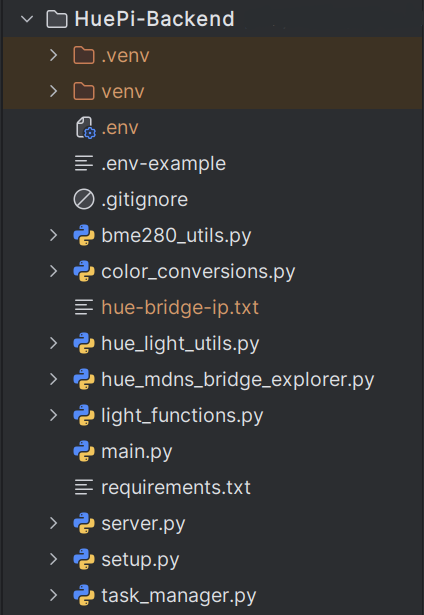
\includegraphics[scale=0.8]{figures/struktura-plikow-raspberry-pi.png}
    \caption{Struktura plików serwera Raspberry Pi}
    \label{fig:struktura-plików-raspberry}
\end{figure}

\subsubsection{.env-example/.env}
\begin{lstlisting}
hue-application-key=abcdefg123456
server-api-key=xyz123
\end{lstlisting}

Pliki \texttt{.env} oraz \texttt{.env-example} są istotnym elementem konfiguracji serwera uruchamianego na Raspberry Pi, zapewniającym bezpieczeństwo oraz łatwość
w zarządzaniu kluczami i danymi dostępowymi. Plik \texttt{.env-example} to przykładowy plik wzorcowy, który definiuje, jakie dane konfiguracyjne powinny znaleźć się
w pliku \texttt{.env}. Zawiera klucze środowiskowe oraz przykładowe wartości, służące jako instrukcja dla użytkownika, który konfiguruje serwer. Plik \texttt{.env}
to właściwy plik konfiguracyjny, używany podczas uruchamiania serwera. Zawiera rzeczywiste wartości kluczy, które są wymagane do działania serwera. W projekcie pełni
następujące funkcje:

\begin{itemize}
    \item \texttt{hue-application-key} – przechowuje klucz aplikacji Philips Hue, który jest niezbędny do wykonywania zapytań do API mostka Philips Hue. Klucz ten pozwala
          na autoryzację oraz wykonywanie jakichkolwiek poleceń.
    \item \texttt{server-api-key} – klucz autoryzacyjny wymagany przez serwer FastAPI uruchomiony na Raspberry Pi. Każde żądanie do serwera Raspberry Pi musi zawierać ten
          klucz w nagłówku, aby zostało zaakceptowane. Mechanizm ten zabezpiecza serwer przed nieautoryzowanym dostępem.
\end{itemize}
Pliki \texttt{.env} i \texttt{.env-example} są kluczowymi elementami konfiguracji serwera w projekcie. Dzięki nim zarządzanie wrażliwymi danymi, takimi jak klucze API,
jest łatwe, bezpieczne i zgodne z nowoczesnymi standardami tworzenia oprogramowania. Plik \texttt{.env-example} pełni rolę dokumentacji dla użytkowników, podczas gdy plik
\texttt{.env} zawiera rzeczywiste wartości wymagane do uruchomienia serwera.

\clearpage
\subsubsection{setup.py}
\begin{lstlisting}[language=Python]
    import hue_mdns_bridge_explorer
    
    hue_bridge_explorer = hue_mdns_bridge_explorer.HueBridgeListener()
    
    def init():
        print("Looking for Philips Hue bridges...")
        hue_bridge_ip_addresses_list = hue_mdns_bridge_explorer.get_hue_bridge_ips()
        if len(hue_bridge_ip_addresses_list) > 1:
            print("More than 1 Hue bridge found! Terminating...")
            quit(0)
        elif len(hue_bridge_ip_addresses_list) == 0:
            print("No Hue bridge found! Terminating...")
            quit(0)
        else:
            with open("hue-bridge-ip.txt", "w") as file:
                file.write(str(hue_bridge_ip_addresses_list[0]))
                print(f"Hue Bridge found! Its IP address set to: {str(hue_bridge_ip_addresses_list[0])}")
\end{lstlisting}
Plik \texttt{setup.py} pełni kluczową rolę w procesie inicjalizacji serwera na Raspberry Pi, umożliwiając automatyczne wykrycie mostka Philips Hue w sieci lokalnej i
zapisanie jego adresu IP w pliku konfiguracyjnym. Jest to istotny krok w przygotowaniu środowiska pracy, ponieważ adres IP mostka jest wymagany do komunikacji z jego API.

\subsubsection*{Funkcjonalność pliku \texttt{setup.py}}
\begin{itemize}
    \item \textbf{Wykrywanie mostków Philips Hue:} Plik wykorzystuje skrypt\\\texttt{hue\_mdns\_bridge\_explorer.py}, który przy pomocy protokołu mDNS przeszukuje
          sieć lokalną w celu odnalezienia mostków Philips Hue.
    \item \textbf{Zapis adresu IP:} Po wykryciu mostka jego adres IP jest zapisywany w pliku \texttt{hue-bridge-ip.txt}, który jest później używany przez inne skrypty,
          takie jak \texttt{server.py}, do komunikacji z mostkiem.
    \item \textbf{Walidacja wyników:} Plik sprawdza, ile mostków zostało wykrytych. Jeśli znaleziono więcej niż jeden mostek lub żadnego, proces zostaje zatrzymany,
          a użytkownik jest o tym informowany.
\end{itemize}

\subsubsection*{Działanie krok po kroku}
\begin{itemize}
    \item \textbf{Wykrywanie mostków:} Funkcja \texttt{init()} korzysta z metody\\\texttt{get\_hue\_bridge\_ips()} zaimplementowanej w pliku \texttt{hue\_mdns\_bridge\_explorer.py},
    aby znaleźć dostępne mostki Hue w sieci lokalnej.
    \item \textbf{Sprawdzenie liczby mostków:} Jeśli nie znaleziono żadnych mostków lub wykryto ich więcej niż jeden, skrypt kończy działanie, wyświetlając stosowny komunikat. 
    \item \textbf{Zapis adresu IP:} W przypadku wykrycia dokładnie jednego mostka jego adres IP jest zapisywany w pliku \texttt{hue-bridge-ip.txt}, aby mógł być później używany przez inne skrypty.
\end{itemize}
Plik \texttt{setup.py} automatyzuje proces inicjalizacji serwera, zapewniając poprawne skonfigurowanie środowiska pracy. Dzięki automatycznemu wykrywaniu mostka Hue
izapisowi jego adresu IP, minimalizuje ryzyko błędów ręcznej konfiguracji oraz upraszcza proces uruchamiania projektu.

\subsubsection{hue\_mdns\_bridge\_explorer.py}
\begin{lstlisting}[language=Python]
from zeroconf import ServiceBrowser, Zeroconf
import socket
import time

class HueBridgeListener:
    def __init__(self):
        self.hue_bridge_ips = []

    def remove_service(self, zeroconf: Zeroconf, type_: str, name: str) -> None:
        pass

    def add_service(self, zeroconf: Zeroconf, type_: str, name: str) -> None:
        info = zeroconf.get_service_info(type_, name)
        if info:
            ip_ = socket.inet_ntoa(info.addresses[0])
            self.hue_bridge_ips.append(ip_)

    def update_service(self, zeroconf: Zeroconf, type_: str, name: str) -> None:
        pass

def find_hue_bridges():
    zeroconf = Zeroconf()
    _listener = HueBridgeListener()
    browser = ServiceBrowser(zeroconf, "_hue._tcp.local.", _listener)
    time.sleep(5)
    zeroconf.close()
    return _listener.hue_bridge_ips

def get_hue_bridge_ips():
    _bridges = find_hue_bridges()
    return _bridges

if __name__ == '__main__':
    listener = HueBridgeListener()
    bridges = get_hue_bridge_ips()
    for bridge in bridges:
        print(bridge)
\end{lstlisting}

Plik \texttt{hue\_mdns\_bridge\_explorer.py} odpowiada za wyszukiwanie mostków Philips Hue w sieci lokalnej przy użyciu protokołu mDNS (\textit{Multicast DNS}).
Jest kluczowym komponentem systemu, ponieważ umożliwia dynamiczne wykrywanie urządzeń, eliminując potrzebę ręcznego wprowadzania adresu IP mostka.

\subsubsection*{Funkcjonalność pliku \texttt{hue\_mdns\_bridge\_explorer.py}}
\begin{itemize}
    \item \textbf{Przeszukiwanie sieci lokalnej w poszukiwaniu mostków Hue:} Wykorzystuje protokół mDNS do odnajdywania urządzeń, które ogłaszają swoje usługi pod nazwą
    \texttt{\_hue.\_tcp.local.}
    \item \textbf{Pobieranie adresów IP wykrytych mostków:} Gdy mostek Hue zostanie wykryty, jego adres IP jest dodawany do listy dostępnych urządzeń.
    \item \textbf{Obsługa dynamicznych zmian w sieci:} Skrypt nasłuchuje zmiany w dostępnych usługach, dzięki czemu może na bieżąco aktualizować listę wykrytych urządzeń.
\end{itemize}


\subsubsection*{Działanie krok po kroku}
\begin{itemize}
    \item \textbf{Inicjalizacja klasy \texttt{HueBridgeListener}:} Klasa ta jest odpowiedzialna za nasłuchiwanie usług w sieci lokalnej i zapisywanie adresów IP wykrytych mostków Hue.
    \item \textbf{Obsługa zdarzeń:} Metody \texttt{add\_service()}, \texttt{remove\_service()} oraz \texttt{update\_service()} reagują na zmiany w dostępnych usługach sieciowych.
    \item \textbf{Wyszukiwanie mostków:} Funkcja \texttt{find\_hue\_bridges()} używa obiektu \texttt{Zeroconf} do przeszukiwania sieci pod kątem usług \texttt{\_hue.\_tcp.local.} i pobiera ich adresy IP.
    \item \textbf{Udostępnienie listy mostków:} Funkcja \texttt{get\_hue\_bridge\_ips()} zwraca listę wykrytych adresów IP mostków Philips Hue.
    \item \textbf{Uruchomienie skryptu:} Jeśli plik jest uruchamiany jako główny moduł, skrypt wypisuje na ekranie znalezione mostki.
\end{itemize}
Plik \texttt{hue\_mdns\_bridge\_explorer.py} jest wykorzystywany przez inne komponenty systemu, takie jak \texttt{setup.py}, do dynamicznego wykrywania mostka Hue.
Dzięki zastosowaniu protokołu mDNS użytkownik nie musi ręcznie konfigurować adresu IP urządzenia, co znacząco ułatwia proces instalacji i konfiguracji.

\subsubsection{color\_conversions.py}
\begin{lstlisting}[language=Python]
from rgbxy import Converter
from rgbxy import GamutC
from colorsys import hsv_to_rgb

converter = Converter(GamutC)


def hsv2rgb(h, s, v):
    """Converts hsv(0-1, 0-1, 0-1) to rgb in 0-255 range"""
    return tuple(round(i * 255) for i in hsv_to_rgb(h, s, v))


def hsv2xy(h, s, v):
    """Converts hsv (0-1, 0-1, 0-1 ranges) to Philips' Hue xy values (0-1, 0-1)"""
    _v = v
    if v <= 0.001:
        _v = 0.01
    r, g, b = hsv2rgb(h, s, _v)
    x, y = converter.rgb_to_xy(r, g, b)
    return x, y


def rgb2xy(r, g, b):
    """Converts rgb(0-255, 0-255, 0-255) to Philips' Hue xy values"""
    if r == 0 and g == 0 and b == 0:
        return 0, 0
    x, y = converter.rgb_to_xy(r, g, b)
    return x, y

def xy2hex(x, y):
    """Converts Philips' Hue xy to hex"""
    hex = converter.xy_to_hex(x, y)
    return hex

if __name__ == '__main__':
    print(rgb2xy(255, 0, 255))
\end{lstlisting}
Plik \texttt{color\_conversions.py} zawiera zestaw funkcji umożliwiających konwersję kolorów pomiędzy różnymi modelami, takimi jak HSV, RGB i XY. Jest to niezbędne w kontekście integracji
z systemem Philips Hue, ponieważ mostek Hue operuje na współrzędnych barwowych \texttt{x} i \texttt{y}, zamiast standardowych wartości RGB czy HSV. Do tego różne modele żarówek Philips Hue posiadają
różne tzw. \textit{gamuty} co jeszcze bardziej komplikuje konwersję kolorów. Do pomocy przy konwersji została użyta bibliteka \textbf{rgbxy}.
Główne funkcje w tym pliku odpowiadają za konwersję kolorów z modelu HSV na RGB, a następnie na wartości \texttt{x, y}, które mogą być przesłane do API Philips Hue. Dodatkowo umożliwiają
przekształcenie barw zapisanych w formacie RGB bezpośrednio do współrzędnych \texttt{xy}, co pozwala na precyzyjne odwzorowanie kolorów w inteligentnym oświetleniu. Oprócz tego dostępna jest
funkcja zamieniająca wartości \texttt{x, y} na reprezentację heksadecymalną, co może być przydatne do wizualizacji aktualnych ustawień oświetlenia. Plik ten zapewnia kompatybilność między
różnymi modelami kolorów i eliminuje konieczność ręcznego przeliczania wartości, co znacząco ułatwia implementację funkcji zmiany barw w systemie sterowania oświetleniem.


\subsubsection{bme280\_utils.py}
\begin{lstlisting}[language=Python]
import bme280
import smbus2

port = 1
address = 0x76
bus = smbus2.SMBus(port)

bme280.load_calibration_params(bus, address)


def read_temperature():
    data = bme280.sample(bus, address)
    return round(data.temperature, 3)


def read_pressure():
    data = bme280.sample(bus, address)
    return round(data.pressure, 3)


def read_humidity():
    data = bme280.sample(bus, address)
    return round(data.humidity, 3)

\end{lstlisting}
Plik \texttt{bme280\_utils.py} zawiera funkcje umożliwiające odczyt danych z czujnika BME280, który mierzy temperaturę, ciśnienie atmosferyczne oraz wilgotność. Komunikacja z czujnikiem odbywa
się za pośrednictwem magistrali I²C przy użyciu biblioteki \texttt{bme280}. Skrypt inicjalizuje czujnik, ładuje parametry kalibracyjne, a następnie dostarcza trzy główne funkcje:
\texttt{read\_temperature()}, \texttt{read\_pressure()} oraz \texttt{read\_humidity()}, które zwracają aktualne wartości pomiarowe. Dane te mogą być wykorzystywane np. do dynamicznej zmiany
ustawień oświetlenia w zależności od temperatury lub do monitorowania warunków środowiskowych. Plik ten pełni kluczową rolę w integracji systemu z rzeczywistymi danymi atmosferycznymi,
pozwalając na ich łatwe pobieranie i dalsze przetwarzanie przez inne moduły aplikacji.



\subsubsection{hue\_light\_utils.py}
\begin{lstlisting}[language=Python]
import requests as rq
import json
import urllib3
from color_conversions import xy2hex
urllib3.disable_warnings(urllib3.exceptions.InsecureRequestWarning)


def check_response(response: rq.Response):
    if (response.status_code != 200) and (response.status_code != 207):
        print(f'There is something wrong with the Philips Hue API call! Status code: {response.status_code}')


def powered_on(header, light_id, bridge_ip):
    light_url = f"https://{bridge_ip}/clip/v2/resource/light/{light_id}"
    r = rq.get(url=light_url, headers=header, verify=False)
    check_response(r)
    response_json = r.json()
    light_on = response_json['data'][0]['on']['on']
    if light_on:
        return True
    else:
        return False


def switch_power(header, light_id, bridge_ip):
    light_url = f"https://{bridge_ip}/clip/v2/resource/light/{light_id}"
    payload_on = json.dumps({
        "on": {
            "on": True
        }
    })

    payload_off = json.dumps({
        "on": {
            "on": False
        }
    })
    if powered_on(header, light_id, bridge_ip):
        r = rq.put(url=light_url, headers=header, data=payload_off, verify=False)
        check_response(r)
        return {"message": "OK"}
    else:
        r = rq.put(url=light_url, headers=header, data=payload_on, verify=False)
        check_response(r)
        return {"message": "OK"}


def turn_on(header, light_id, bridge_ip):
    if powered_on(header, light_id, bridge_ip):
        return {"message": "Already turned on!"}
    else:
        light_url = f"https://{bridge_ip}/clip/v2/resource/light/{light_id}"
        payload = json.dumps({
            "on": {
                "on": True
            }
        })
        r = rq.put(url=light_url, headers=header, data=payload, verify=False)
        check_response(r)
        return {"message": "OK"}


def turn_off(header, light_id, bridge_ip):
    if not powered_on(header, light_id, bridge_ip):
        return {"message": "Already turned off!"}
    else:
        light_url = f"https://{bridge_ip}/clip/v2/resource/light/{light_id}"
        payload = json.dumps({
            "on": {
                "on": False
            }
        })
        r = rq.put(url=light_url, headers=header, data=payload, verify=False)
        check_response(r)
        return {"message": "OK"}


def change_brightness(header, light_id, level, bridge_ip):
    level_int = (round(level, 2) * 100)

    if level_int > 100:
        level_int = 100
    elif level_int < 0:
        level_int = 0

    light_url = f"https://{bridge_ip}/clip/v2/resource/light/{light_id}"
    payload = json.dumps({
        "dimming": {
            "brightness": level_int
        }
    })
    r = rq.put(url=light_url, headers=header, data=payload, verify=False)
    check_response(r)
    return {"message": "OK"}


def change_color(header, light_id, bridge_ip, x, y):
    light_url = f"https://{bridge_ip}/clip/v2/resource/light/{light_id}"
    r = rq.put(url=light_url, headers=header,
                json={
                    "color": {
                        "xy": {
                            "x": x,
                            "y": y
                        }
                    }
                }, verify=False)
    check_response(r)
    return {"message": "OK"}


def get_full_lights(header, bridge_ip):
    base_url = f"https://{bridge_ip}/clip/v2/resource"
    devices_url = f"{base_url}/device"
    
    # First GET request to retrieve all light devices which returns only "rid" and "name" 
    response = rq.get(url=devices_url, headers=header, verify=False)
    lights = []
    
    check_response(response)
    
    response_data = response.json()
    for device in response_data.get("data", []):
        for service in device.get("services", []):
            if service.get("rtype") == "light":
                light_rid = service["rid"]
                
                # Second GET request for detailed light information
                light_url = f"{base_url}/light/{light_rid}"
                light_response = rq.get(url=light_url, headers=header, verify=False)
                
                if (light_response.status_code != 200 and light_response.status_code != 207):
                    print("Error fetching light details:", light_response.status_code, light_response.text)
                    brightness = None
                    is_on: bool = None
                    color_hex = None

                light_data = light_response.json().get("data", [])[0]
                brightness = light_data.get("dimming", {}).get("brightness")
                is_on = light_data.get("on", {}).get("on")
                xy_color = light_data.get("color", {}).get("xy")
                color_hex = xy2hex(xy_color["x"], xy_color["y"]) if xy_color else None
                name = device["metadata"]["name"]

                light_info = {
                    "rid": light_rid,
                    "name": name,
                    "brightness": brightness,
                    "isOn": is_on,
                    "color": f"#{color_hex}",
                }
                lights.append(light_info)
    return lights


def get_light_details(header, bridge_ip, light_id):
    light_url = f"https://{bridge_ip}/clip/v2/resource/light/{light_id}"
    response = rq.get(url=light_url, headers=header, verify=False)
    
    print(response.status_code)
    if (response.status_code != 200 and response.status_code != 207):
        print("Error fetching light details:", response.status_code, response.text)
        return None

    light_data = response.json().get("data", [])[0]  # Get the first light data object
    
    brightness_float_100_range = light_data.get("dimming", {}).get("brightness")
    brightness_float_1_range = round((brightness_float_100_range/100), 2)
    name = light_data.get("metadata", {}).get("name")
    is_on = light_data.get("on", {}).get("on")
    xy_color = light_data.get("color", {}).get("xy")
    color_hex = xy2hex(xy_color["x"], xy_color["y"]) if xy_color else None


    light_info = {
        "rid": light_id,
        "name": name,
        "brightness": brightness_float_1_range,
        "isOn": is_on,
        "color": f"#{color_hex}",
    }

    return light_info
    
\end{lstlisting}
Plik \texttt{hue\_light\_utils.py} zawiera zestaw funkcji odpowiedzialnych za komunikację serwera z mostkiem Philips Hue poprzez jego API. Definiuje zapytania HTTP umożliwiające sterowanie
inteligentnym oświetleniem, w tym włączanie i wyłączanie świateł, zmianę jasności, kolorów oraz pobieranie szczegółowych informacji o stanie poszczególnych źródeł światła. Wszystkie operacje są
realizowane za pomocą żądań \texttt{GET} i \texttt{PUT}, wysyłanych do odpowiednich endpointów mostka Philips Hue. Plik wykorzystuje bibliotekę \texttt{requests} do obsługi połączeń HTTP, a
także umożliwia konwersję danych kolorystycznych do formatu \texttt{xy}, wymaganego przez API Hue. Dodatkowo zawiera funkcję sprawdzającą odpowiedzi serwera i informującą o ewentualnych błędach
w komunikacji. Moduł ten stanowi kluczowy element systemu sterowania oświetleniem, pozwalając na łatwą integrację funkcji związanych z inteligentnym oświetleniem oraz zapewniając płynną komunikację
między serwerem a urządzeniami Hue.

\subsubsection{light\_functions.py}
\begin{lstlisting}[language=Python]
def translate_temperature_to_hsv_color(input_temp, temp_min, temp_max, hsv_color_min, hsv_color_max):
if input_temp <= temp_min:
    return hsv_color_min
if input_temp >= temp_max:
    return hsv_color_max

# Determine the range of the input temperatures
temp_span = temp_max - temp_min

# Scale the temperature into a 0-1 range
value_scaled = float(input_temp - temp_min) / float(temp_span)

# Handle the circular nature of the hue
if hsv_color_min <= hsv_color_max:
    # Normal case, no wrapping needed
    hue_color_span = hsv_color_max - hsv_color_min
    return hsv_color_min + (value_scaled * hue_color_span)
else:
    # Wrapping case
    hue_color_span = (1 - hsv_color_min) + hsv_color_max
    hue = hsv_color_min + (value_scaled * hue_color_span)
    if hue > 1:  # Wrap around the circle
        hue -= 1
    return hue
\end{lstlisting}
Plik \texttt{light\_functions.py} zawiera funkcję umożliwiającą dynamiczne przekształcanie temperatury otoczenia na wartość koloru w przestrzeni HSV. Funkcja\\ \texttt{translate\_temperature\_to\_hsv\_color()}
przyjmuje wartości minimalnej i maksymalnej temperatury oraz odpowiadające im kolory w modelu HSV. Na tej podstawie dokonuje interpolacji, aby dla danej temperatury zwrócić odpowiednią wartość koloru,
uwzględniając cykliczną naturę skali barw HSV. Moduł ten umożliwia tworzenie dynamicznych efektów świetlnych opartych na rzeczywistych danych pomiarowych, co pozwala na inteligentne dostosowanie
oświetlenia do aktualnych warunków otoczenia.

\subsubsection{task\_manager.py}
\begin{lstlisting}[language=Python]
class TaskManager:
def __init__(self):
    self.tasks = {}

def start_task(self, light_id: str, task: callable, *args, **kwargs):
    if light_id in self.tasks:
        raise ValueError(f"A task is already running for light_id {light_id}.")
    self.tasks[light_id] = True
    task(*args, **kwargs)

def stop_task(self, light_id: str):
    if light_id in self.tasks:
        self.tasks[light_id] = False
        del self.tasks[light_id]

def is_task_running(self, light_id: str) -> bool:
    return self.tasks.get(light_id, False)


task_manager = TaskManager()
\end{lstlisting}
Plik \texttt{task\_manager.py} zawiera implementację klasy \texttt{TaskManager}, która odpowiada za zarządzanie zadaniami wykonywanymi w tle. Klasa ta umożliwia uruchamianie, zatrzymywanie oraz
monitorowanie zadań związanych ze sterowaniem oświetleniem Philips Hue. \texttt{TaskManager} przechowuje informacje o aktualnie wykonywanych procesach dla poszczególnych świateł, zapobiegając
ich jednoczesnemu uruchamianiu. Jest to szczególnie istotne w kontekście dynamicznych funkcji, takich jak automatyczna zmiana koloru w zależności od temperatury. Klasa ta jest wykorzystywana w pliku
\texttt{server.py}, gdzie pozwala na kontrolowanie działania długotrwałych procesów związanych z oświetleniem. Dzięki niej możliwe jest bezpieczne i kontrolowane zarządzanie stanem świateł,
bez ryzyka kolizji między operacjami.

\subsubsection{server.py}
Plik \texttt{server.py} stanowi główną część serwera aplikacji, który został zbudowany przy użyciu frameworka FastAPI. Serwer ten obsługuje żądania HTTP i umożliwia komunikację między klientem
a mostkiem Philips Hue, umożliwiając sterowanie inteligentnym oświetleniem. Plik integruje różne moduły, w tym \texttt{hue\_light\_utils.py} do wysyłania żądań do mostka Hue, \texttt{bme280\_utils.py}
do pobierania danych z czujnika BME280 oraz \texttt{task\_manager.py} do zarządzania długotrwałymi procesami. Serwer implementuje mechanizm uwierzytelniania za pomocą klucza API, co zabezpiecza
dostęp do funkcji sterujących oświetleniem. Obsługuje różne operacje, takie jak włączanie i wyłączanie świateł, zmiana ich jasności, kolorów oraz dynamiczne dostosowywanie barwy światła na podstawie temperatury. 

\subsubsection*{Przykładowa funkcja: \texttt{turn\_on()}}
\noindent Jednym z endpointów dostępnych w serwerze jest funkcja \texttt{turn\_on()}, która odpowiada za włączanie światła o określonym identyfikatorze. 

\begin{lstlisting}[language=Python]
@app.get("/turn-on/{light_id}")
async def turn_on(light_id: str, api_key: str = Security(get_api_key)):
    _header = {"hue-application-key": hue_api_key}
    response = hue_light_utils.turn_on(header=_header, light_id=light_id, bridge_ip=hue_bridge_ip_address)
    if response.get("message") == "OK":
        return {"message": "Turned on!"}
    elif response.get("message") == "Already turned on!":
        return {"message": "Already turned on!"}
    else:
        return {"message": "Something's wrong!"}, 500
\end{lstlisting}
Funkcja ta przyjmuje identyfikator światła jako parametr ścieżki oraz sprawdza poprawność klucza API. Następnie tworzy nagłówek uwierzytelniający, który jest wymagany przez mostek Hue,
i wywołuje metodę \texttt{turn\_on()} zdefiniowaną w \texttt{hue\_light\_utils.py}. Na podstawie odpowiedzi API zwraca komunikat informujący o powodzeniu operacji lub ewentualnym błędzie.\\
Plik \texttt{server.py} pełni rolę centralnego elementu aplikacji, umożliwiającego komunikację między klientem a mostkiem Philips Hue. Dzięki zastosowaniu FastAPI i podziałowi na moduły
zapewnia wydajną obsługę żądań oraz elastyczność w zarządzaniu inteligentnym oświetleniem.

\clearpage
\subsubsection{ main.py}
\begin{lstlisting}[language=Python]
import subprocess
import setup
import hue_mdns_bridge_explorer

if __name__ == "__main__":
    hue_bridge_explorer = hue_mdns_bridge_explorer.HueBridgeListener()
    setup.init()

    command = [
        "uvicorn",
        "server:app",
        "--host", "0.0.0.0",
        "--port", "8000",
    ]

    print(f"Running command: \"{' '.join(command)}\"")

    subprocess.run(command, check=True)
\end{lstlisting}
Plik \texttt{main.py} pełni rolę punktu wejściowego do uruchomienia serwera aplikacji. Jego zadaniem jest przygotowanie środowiska, w tym inicjalizacja konfiguracji mostka Philips Hue,
a następnie uruchomienie serwera FastAPI. Na początku skrypt wywołuje funkcję \texttt{init()} z pliku \texttt{setup.py}, która automatycznie wykrywa adres IP mostka Philips Hue i zapisuje
go w pliku konfiguracyjnym. Następnie definiowana jest komenda do uruchomienia serwera przy użyciu frameworka \texttt{Uvicorn}, który jest asynchronicznym serwerem HTTP przeznaczonym do obsługi
aplikacji FastAPI. Serwer zostaje uruchomiony na wszystkich interfejsach sieciowych urządzenia (\texttt{0.0.0.0}) na porcie 8000. Po wykryciu mostka Hue i zapisaniu jego adresu IP, skrypt uruchamia
serwer FastAPI, który nasłuchuje na porcie 8000. Dzięki temu serwer jest gotowy do obsługi zapytań związanych ze sterowaniem oświetleniem.

Plik \texttt{main.py} pełni funkcję inicjalizacyjną i uruchamiającą serwer aplikacji. Automatyzuje proces konfiguracji mostka Philips Hue oraz uruchamia serwer FastAPI, zapewniając gotowe
środowisko do obsługi żądań HTTP związanych ze sterowaniem inteligentnym oświetleniem.

\clearpage

\subsection{Aplikacja mobilna}
Poniższy \hyperlink{fig:struktura-plików-aplikacja-mobilna}{rysunek} przedstawia strukturę plików projektu.

\begin{figure}[H]
    \centering
    \hypertarget{fig:struktura-plików-aplikacja-mobilna}{}
    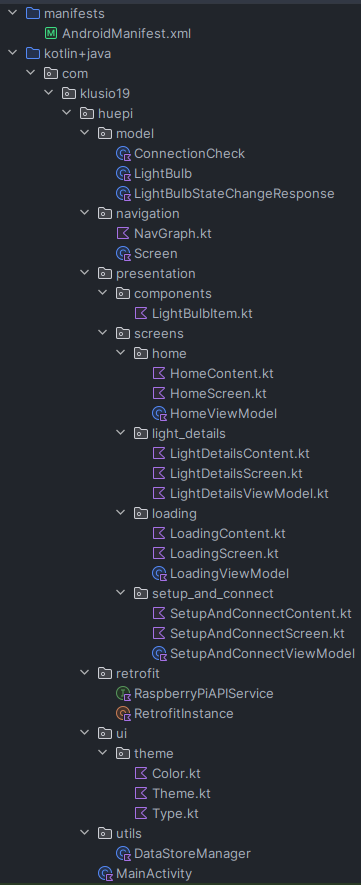
\includegraphics[scale=0.8]{figures/struktura-plikow-aplikacja-mobilna.png}
    \caption{Struktura plików projektu aplikacji mobilnej}
    \label{fig:struktura-plików-raspberry}
\end{figure}


Aplikacja mobilna HuePi została stworzona w języku Kotlin i wykorzystuje nowoczesne technologie oraz wzorce projektowe stosowane w aplikacjach na system Android. Jej głównym
celem jest umożliwienie użytkownikowi wygodnego sterowania inteligentnym oświetleniem Philips Hue poprzez komunikację z serwerem uruchomionym na Raspberry Pi. 

\subsubsection*{Architektura aplikacji}
Aplikacja została zaprojektowana zgodnie z wzorcem \textit{MVVM (Model-View-ViewModel)}, który zapewnia lepszą separację logiki biznesowej od interfejsu użytkownika. Struktura kodu została podzielona na trzy główne warstwy:
\begin{itemize}
    \item \textbf{Model} – zawiera definicje klas danych, takich jak reprezentacje żarówek (\texttt{LightBulb.kt}) oraz odpowiedzi serwera na zmiany stanu świateł.
    \item \textbf{View} – oparta na \textbf{Jetpack Compose}, odpowiada za warstwę interfejsu użytkownika, umożliwiając dynamiczne tworzenie widoków w sposób deklaratywny.
    \item \textbf{ViewModel} – pośredniczy między widokiem a warstwą modelu, zarządza stanem aplikacji i obsługuje logikę biznesową.
\end{itemize}

\subsubsection*{Interfejs użytkownika – Jetpack Compose}
Do budowy interfejsu aplikacji wykorzystano \textbf{Jetpack Compose}, który umożliwia deklaratywne definiowanie komponentów UI oraz elastyczne zarządzanie stanem. Dzięki temu
aplikacja jest bardziej responsywna, a kod jest czytelniejszy i łatwiejszy w utrzymaniu w porównaniu do tradycyjnego podejścia opartego na plikach XML.

\subsubsection*{Komunikacja z serwerem Raspberry Pi}
Aplikacja wykorzystuje bibliotekę \textbf{Retrofit}, aby komunikować się z serwerem uruchomionym na Raspberry Pi, który zarządza mostkiem Philips Hue oraz czujnikiem BME280. Wysyłane żądania HTTP pozwalają na:
\begin{itemize}
    \item włączanie i wyłączanie żarówek,
    \item zmianę jasności oraz koloru świateł,
    \item odczytywanie aktualnego stanu żarówek,
\end{itemize}

\subsubsection*{Obsługa nawigacji}
Za zarządzanie przejściami między ekranami odpowiada moduł \textbf{Jetpack Compose Navigation}, który definiuje dostępne ścieżki oraz obsługuje przechodzenie między poszczególnymi ekranami
aplikacji. Każdy ekran aplikacji został wydzielony do osobnego modułu w katalogu \texttt{presentation/screens}, co ułatwia organizację kodu oraz jego rozbudowę.

\subsubsection*{Przechowywanie danych}
Do zarządzania lokalnymi ustawieniami aplikacji wykorzystano bibliotekę \textbf{DataStore Preferences}, która zastępuje starszy mechanizm \textit{SharedPreferences}.
Pozwala to na bezpieczne i wydajne przechowywanie preferencji użytkownika, takich jak ostatnio wybrana żarówka czy stan połączenia z serwerem.

\subsubsection*{Struktura aplikacji}
\noindent Aplikacja została podzielona na logiczne moduły, w tym:
\begin{itemize}
    \item \texttt{model} – definiuje struktury danych wykorzystywane w aplikacji,
    \item \texttt{presentation} – zawiera komponenty UI oraz ekrany aplikacji,
    \item \texttt{retrofit} – obsługuje komunikację z serwerem przy użyciu Retrofit,
    \item \texttt{navigation} – odpowiada za system nawigacji pomiędzy ekranami,
    \item \texttt{utils} – zawiera klasy pomocnicze, takie jak \texttt{DataStoreManager} do obsługi ustawień użytkownika,
    \item \texttt{ui/theme} – definiuje motyw graficzny aplikacji (kolory, typografia, styl komponentów UI).
\end{itemize}
Aplikacja \texttt{HuePi} łączy nowoczesne technologie Androida, takie jak \textbf{Jetpack Compose}, \textbf{MVVM}, \textbf{Retrofit} i \textbf{DataStore}, aby zapewnić wygodne
sterowanie inteligentnym oświetleniem. Dzięki modularnej budowie kod aplikacji jest czytelny, łatwy do rozwijania i zgodny z najlepszymi praktykami tworzenia aplikacji mobilnych.

\vspace{\baselineskip}
\noindent Poniżej, w najbliższych podrozdziałach, zostaną omówione poszczególne pliki wchodzące w skład projektu.
\clearpage

\subsubsection{MainActivity.kt}
\begin{lstlisting}[language=Kotlin]
package com.klusio19.huepi

import android.os.Bundle
import androidx.activity.ComponentActivity
import androidx.activity.compose.setContent
import androidx.activity.enableEdgeToEdge
import androidx.core.splashscreen.SplashScreen.Companion.installSplashScreen
import androidx.core.view.WindowCompat
import androidx.navigation.compose.rememberNavController
import com.klusio19.huepi.navigation.Screen
import com.klusio19.huepi.navigation.SetupNavGraph
import com.klusio19.huepi.ui.theme.HuePiTheme

class MainActivity : ComponentActivity() {

    override fun onCreate(savedInstanceState: Bundle?) {
        super.onCreate(savedInstanceState)
        installSplashScreen()
        enableEdgeToEdge()
        WindowCompat.setDecorFitsSystemWindows(window, false)
        setContent {
            HuePiTheme {
                val navController = rememberNavController()
                    SetupNavGraph(
                        startDestination = Screen.Loading,
                        navController = navController,
                        context = application
                    )
            }
        }
    }
}
\end{lstlisting}
Plik \texttt{MainActivity.kt} stanowi główny punkt wejściowy aplikacji \texttt{HuePi}. Jest to jedyna aktywność (\textit{Activity}) w aplikacji, co wynika z zastosowania
\textbf{Jetpack Compose}, który eliminuje konieczność korzystania z wielu aktywności i zamiast tego pozwala na budowanie całego interfejsu użytkownika w sposób deklaratywny
w obrębie jednej aktywności. Głównym zadaniem tej klasy jest inicjalizacja interfejsu użytkownika oraz uruchomienie systemu nawigacji pomiędzy ekranami aplikacji.
Główne zadania \texttt{MainActivity.kt} to:
\begin{itemize}
    \item \textbf{Inicjalizacja aplikacji} – ustawienie motywu i uruchomienie głównej zawartości aplikacji.
    \item \textbf{Zarządzanie nawigacją} – wykorzystanie Jetpack Navigation do obsługi przejść między ekranami.
    \item \textbf{Obsługa stanu aplikacji} – przekazywanie odpowiednich obiektów \texttt{ViewModel} do ekranów, które tego wymagają.
\end{itemize}

\subsubsection{NavGraph.kt}
Plik \texttt{NavGraph.kt} odpowiada za zarządzanie nawigacją w aplikacji \texttt{HuePi}. Wykorzystuje on bibliotekę \textbf{Jetpack Compose Navigation}, dostosowaną do deklaratywnego
podejścia stosowanego w \textbf{Jetpack Compose}. Ponieważ cała aplikacja działa w jednej aktywności, wszystkie ekrany są obsługiwane dynamicznie w ramach systemu nawigacji.

Plik definiuje główny kontener nawigacyjny \texttt{NavHost}, który przechowuje listę dostępnych ekranów i zarządza ich zmianą. Struktura nawigacji opiera się na koncepcji
\textbf{grafu nawigacyjnego}, w którym każda ścieżka (route) reprezentuje jeden z ekranów aplikacji. Dzięki temu podejściu przejścia pomiędzy ekranami realizowane są poprzez
dynamiczne wywoływanie funkcji \texttt{navigate()} na obiekcie \texttt{NavController}, co pozwala na płynną zmianę widoków w aplikacji.

\subsubsection*{Zasada działania}
Główna funkcja \texttt{SetupNavGraph()} inicjalizuje nawigację, ustawiając ekran startowy oraz rejestrując poszczególne ścieżki. Każdy ekran jest rejestrowany jako osobna
funkcja rozszerzająca \texttt{NavGraphBuilder}, co pozwala na lepszą organizację kodu.

\begin{lstlisting}[language=Kotlin]
@Composable
fun SetupNavGraph(startDestination: Screen, navController: NavHostController, context: Application) {
    NavHost(navController = navController, startDestination = startDestination) {
        loadingRoute(context, navController)
        setupAndConnectRoute(navController)
        homeRoute(navController)
        lightRoute(context)
    }
}
\end{lstlisting}

W ramach \texttt{NavHost} rejestrowane są funkcje obsługujące poszczególne ekrany, takie jak:
\begin{itemize}
    \item \texttt{loadingRoute()} – obsługuje ekran ładowania i przekierowuje użytkownika do odpowiedniego ekranu po zakończeniu procesu inicjalizacji.
    \item \texttt{setupAndConnectRoute()} – odpowiada za ekran konfiguracji połączenia z mostkiem Philips Hue i serwerem Raspberry Pi.
    \item \texttt{homeRoute()} – zarządza ekranem głównym, który wyświetla listę dostępnych żarówek.
    \item \texttt{lightRoute()} – odpowiada za ekran szczegółów dotyczących konkretnej żarówki, pozwalając użytkownikowi na zmianę jej stanu, jasności i koloru.    
\end{itemize}

\subsubsection*{Obsługa nawigacji w ekranach}
Każda z funkcji odpowiadających za poszczególne ekrany implementuje własną logikę nawigacji. Na przykład ekran konfiguracji (\texttt{setupAndConnectRoute()}) reaguje
na zdarzenie poprawnej walidacji połączenia i po krótkim opóźnieniu przechodzi do ekranu głównego:

\begin{lstlisting}[language=Kotlin]
fun NavGraphBuilder.setupAndConnectRoute(navController: NavHostController) {
    composable<Screen.SetupAndConnect> {
        val viewModel: SetupAndConnectViewModel = viewModel()
        LaunchedEffect(Unit) {
            viewModel.navigationEvent.collect { shouldNavigate ->
                if (shouldNavigate) {
                    delay(1000L)
                    navController.navigate(Screen.Home)
                }
            }
        }
        SetupAndConnectScreen(...)
    }
}
\end{lstlisting}

W innych przypadkach nawigacja może być bardziej dynamiczna – np. ekran szczegółów żarówki (\texttt{lightRoute()}) pobiera argumenty przekazane w ścieżce nawigacyjnej
(identyfikator żarówki), a następnie inicjalizuje odpowiedni \texttt{ViewModel}:

\begin{lstlisting}[language=Kotlin]
fun NavGraphBuilder.lightRoute(context: Application) {
    composable<Screen.LightDetails> { backStackEntry ->
        val args = backStackEntry.toRoute<Screen.LightDetails>()
        val viewModelFactory = LightDetailsViewModelFactory(context, args.rid)
        val viewModel: LightDetailsViewModel = viewModel(factory = viewModelFactory)
        LightDetailsScreen(...)
    }
}
\end{lstlisting}
Plik \texttt{NavGraph.kt} odpowiada za zarządzanie ruchem w aplikacji, definiując ścieżki między ekranami i obsługując przejścia. Dzięki zastosowaniu modularnej struktury
oraz powiązania ekranów z odpowiednimi \texttt{ViewModel}, aplikacja może dynamicznie reagować na zmiany stanu i zapewniać użytkownikowi płynne doświadczenie. Podejście to
zwiększa elastyczność kodu i pozwala na łatwiejszą rozbudowę w przyszłości.


\subsubsection{Screen.kt}
\begin{lstlisting}[language=Kotlin]
package com.klusio19.huepi.navigation

import kotlinx.serialization.Serializable

@Serializable
sealed class Screen {
    @Serializable
    data object Loading : Screen()

    @Serializable
    data object SetupAndConnect : Screen()

    @Serializable
    data object Home : Screen()

    @Serializable
    data class LightDetails(val rid: String) : Screen()
}
\end{lstlisting}
Plik \texttt{Screen.kt} definiuje wszystkie ekrany dostępne w aplikacji \texttt{HuePi} i określa ich strukturę w systemie nawigacji. Wykorzystuje do tego \textit{sealed class},
która grupuje ekrany jako zamknięty zbiór obiektów. Dzięki temu każdy ekran jest jednoznacznie identyfikowalny i łatwy do obsługi w grafie nawigacyjnym.

W pliku wyróżniono cztery ekrany:
\begin{itemize}
    \item \texttt{Loading} – ekran ładowania aplikacji,
    \item \texttt{SetupAndConnect} – ekran konfiguracji połączenia,
    \item \texttt{Home} – ekran główny, który wyświetla listę żarówek,
    \item \texttt{LightDetails} – ekran szczegółów żarówki, który wymaga identyfikatora światła jako argumentu.
\end{itemize}
Dzięki takiemu podejściu nawigacja w aplikacji jest bardziej czytelna i bezpieczna, a przekazywanie danych między ekranami odbywa się w uporządkowany sposób.

\clearpage
\subsubsection{RetrofitInstance.kt}
\begin{lstlisting}[language=Kotlin]
package com.klusio19.huepi.retrofit

import com.squareup.moshi.Moshi
import com.squareup.moshi.kotlin.reflect.KotlinJsonAdapterFactory
import okhttp3.Interceptor
import okhttp3.OkHttpClient
import okhttp3.Request
import okhttp3.logging.HttpLoggingInterceptor
import retrofit2.Retrofit
import retrofit2.converter.moshi.MoshiConverterFactory

object RetrofitInstance {
    fun getClient(baseUrl: String, raspberryApiKey: String): RaspberryPiAPIService {
        val moshi = Moshi.Builder()
            .add(KotlinJsonAdapterFactory())
            .build()

        val logging = HttpLoggingInterceptor().setLevel(HttpLoggingInterceptor.Level.BODY)

        val okHttpClient = OkHttpClient.Builder()
            .addInterceptor(logging)
            .addInterceptor(
                Interceptor { chain ->
                    val request: Request = chain.request()
                        .newBuilder()
                        .header("api-key", raspberryApiKey)
                        .build()
                    chain.proceed(request)
                }
            ).build()

        val raspberryPiAPIService: RaspberryPiAPIService by lazy {
            Retrofit.Builder()
                .baseUrl(baseUrl)
                .addConverterFactory(MoshiConverterFactory.create(moshi))
                .client(okHttpClient)
                .build()
                .create(RaspberryPiAPIService::class.java)
        }

        return raspberryPiAPIService
    }
}
\end{lstlisting}
Plik \texttt{RetrofitInstance.kt} odpowiada za konfigurację klienta \textbf{Retrofit}, który umożliwia aplikacji \texttt{HuePi} komunikację z serwerem Raspberry Pi. Jest to kluczowy
element warstwy sieciowej, ponieważ definiuje sposób, w jaki aplikacja wysyła żądania do API i przetwarza odpowiedzi.

\subsubsection*{Funkcjonalność}
\begin{itemize}
    \item Tworzy instancję \texttt{Retrofit} z podanym adresem URL i kluczem API serwera Raspberry Pi.
    \item Używa \textbf{Moshi} jako konwertera do obsługi formatu JSON.
    \item Dodaje \textbf{Interceptor}, który automatycznie dołącza nagłówek z kluczem API do każdego zapytania.
    \item Wykorzystuje \textbf{HttpLoggingInterceptor}, który ułatwia debugowanie żądań HTTP.
\end{itemize}

Plik \texttt{RetrofitInstance.kt} centralizuje konfigurację klienta HTTP, zapewniając jednolite miejsce inicjalizacji połączenia z serwerem. Dzięki temu inne moduły aplikacji mogą łatwo
korzystać z API bez konieczności każdorazowego definiowania konfiguracji Retrofitu.


\subsubsection{RaspberryPiAPIService.kt}
Plik \texttt{RaspberryPiAPIService.kt} definiuje interfejs API, który umożliwia aplikacji \texttt{HuePi} komunikację z serwerem Raspberry Pi poprzez żądania HTTP. Retrofit wykorzystuje 
ten interfejs do automatycznego generowania kodu obsługującego połączenia sieciowe, co upraszcza wysyłanie zapytań oraz odbieranie odpowiedzi.
Interfejs zawiera metody odpowiadające operacjom wykonywanym na inteligentnym oświetleniu Philips Hue, takim jak pobieranie listy żarówek, włączanie i wyłączanie świateł, zmiana jasności
i kolorów oraz zarządzanie dynamiczną zmianą barwy w zależności od temperatury. Każda metoda korzysta z adnotacji \texttt{@GET}, definiując odpowiednie ścieżki endpointów serwera.
Dzięki zastosowaniu \texttt{Response<T>}, każda odpowiedź z serwera jest bezpiecznie obsługiwana, umożliwiając łatwą kontrolę poprawności zwracanych danych. Moduł ten stanowi kluczowy
element warstwy sieciowej aplikacji, zapewniając przejrzystą i efektywną komunikację z serwerem.\\
Przykładowa metoda inerfejsu:
\begin{lstlisting}[language=Kotlin]
@GET("/get-details/{rid}")
suspend fun getLightBulbDetails(
    @Path("rid") rid: String
): Response<LightBulb?>
\end{lstlisting}


\subsubsection{DataStoreManager.kt}
Plik \texttt{DataStoreManager.kt} odpowiada za przechowywanie i pobieranie danych konfiguracyjnych związanych z połączeniem aplikacji \texttt{HuePi} z serwerem Raspberry Pi. Do tego celu
wykorzystano \textbf{DataStore Preferences}, które zastępuje starszy mechanizm \textit{SharedPreferences}, oferując bardziej wydajny i bezpieczny sposób zarządzania danymi.\\
Głównym zadaniem \texttt{DataStoreManager.kt} jest zapis i odczyt kluczowych informacji dotyczących serwera Raspberry Pi:
\begin{itemize}
    \item Adres URL serwera – przechowywany, aby użytkownik nie musiał ponownie wpisywać adresu IP przy każdym uruchomieniu aplikacji.
    \item Klucz API – zapisany lokalnie, aby aplikacja mogła automatycznie uwierzytelniać się przy komunikacji z serwerem.
\end{itemize}

\subsubsection*{Zasada działania}
Plik definiuje obiekt \texttt{preferenceDataStore}, który jest powiązany z kontekstem aplikacji i zarządza przechowywaniem preferencji w lokalnym magazynie danych. Dzięki temu aplikacja może zapisywać
i odczytywać ustawienia nawet po jej ponownym uruchomieniu.

Przykładowo, funkcja zapisu adresu serwera działa w następujący sposób:

\begin{lstlisting}[language=Kotlin]
suspend fun saveRaspberryPiUrl(ipAddressToSave: String) {
    context.preferenceDataStore.edit { preferences ->
        preferences[RASPBERRY_PI_URL] = ipAddressToSave
    }
}
\end{lstlisting}
Podczas zapisu dane są umieszczane w \texttt{DataStore}, a każda wartość jest powiązana z unikalnym kluczem. W podobny sposób działa pobieranie wartości – aplikacja sprawdza, czy adres URL
został zapisany, a jeśli nie, zwraca wartość domyślną. Plik \\\texttt{DataStoreManager.kt} pozwala na automatyczne zapamiętywanie danych o serwerze Raspberry Pi, dzięki czemu użytkownik nie musi
ręcznie wprowadzać ich przy każdym uruchomieniu aplikacji. Jest to kluczowe dla wygody użytkowania oraz zapewnienia płynnej komunikacji z systemem inteligentnego oświetlenia.



\subsubsection{Ekran SetupAndConnect}
Ekran \texttt{SetupAndConnect} jest pierwszym ekranem, na który trafia użytkownik po uruchomieniu aplikacji \texttt{HuePi}. Jego głównym celem jest umożliwienie wprowadzenia danych niezbędnych
do nawiązania połączenia z serwerem uruchomionym na \textbf{Raspberry Pi}, który zarządza mostkiem Philips Hue. Użytkownik musi podać:
\begin{itemize}
    \item Adres IP wraz z numerem portu serwera Raspberry Pi.
    \item Klucz API wymagany do autoryzacji żądań wysyłanych do serwera.
\end{itemize}
Po wprowadzeniu tych danych aplikacja sprawdza poprawność podanych wartości, zapisuje je lokalnie przy użyciu \textbf{DataStore Preferences} i próbuje nawiązać połączenie z serwerem.

\begin{figure}[H]
    \centering
    \hypertarget{fig:setup-screen}{}
    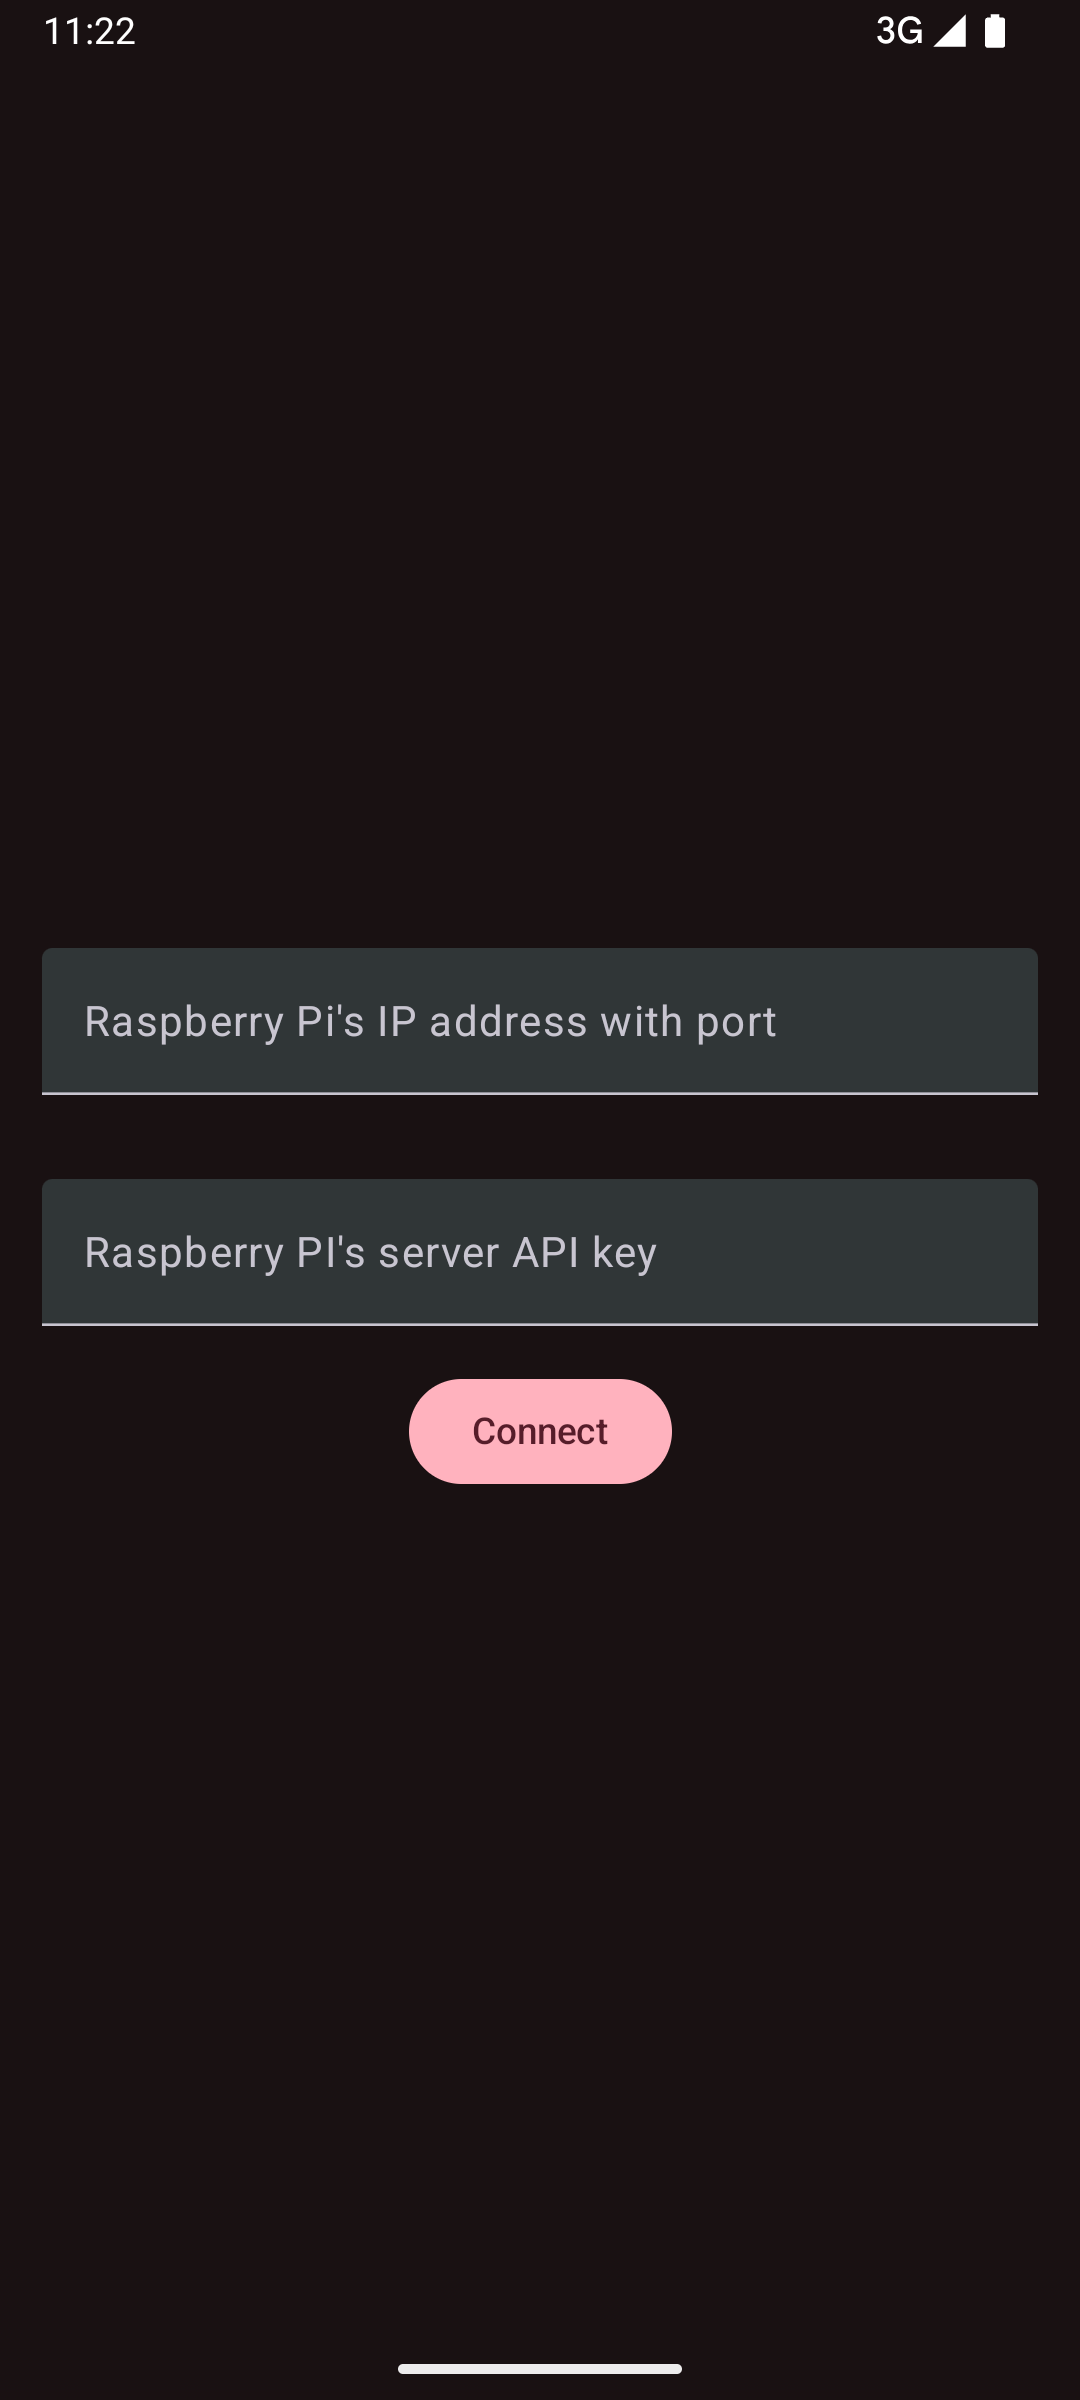
\includegraphics[scale=0.2]{figures/setup_screen.png}
    \caption{Ekran setup\_and\_connect}
    \label{fig:błędne-dane-setup-screen}
\end{figure}

\subsubsection*{Struktura plików ekranu}
\noindent Ekran został podzielony na trzy pliki:
\begin{itemize}
    \item \textbf{\texttt{SetupAndConnectScreen.kt}} – główny kontener ekranu, który ustawia tło aplikacji i wywołuje funkcję odpowiedzialną za zawartość interfejsu.
    \item \textbf{\texttt{SetupAndConnectContent.kt}} – definiuje wygląd i układ komponentów interfejsu użytkownika, takich jak pola tekstowe i przyciski.
    \item \textbf{\texttt{SetupAndConnectViewModel.kt}} – zarządza logiką biznesową, w tym walidacją danych wejściowych oraz nawiązywaniem połączenia z serwerem.
\end{itemize}
Podział ten zgodny jest z architekturą \textit{MVVM} (Model-View-ViewModel), która pozwala na oddzielenie logiki aplikacji od interfejsu użytkownika, co ułatwia testowanie i utrzymanie kodu.

\subsubsection*{Walidacja danych wejściowych}
\noindent Aby uniknąć błędów użytkownika, ekran zawiera prostą walidację danych. Weryfikowane są dwa kluczowe elementy:
\begin{itemize}
    \item Adres IP i port – musi składać się z co najmniej 13 znaków.
    \item Klucz API – nie może być pusty.
\end{itemize}

\noindent Przykładowa implementacja walidacji znajduje się w pliku \\\texttt{SetupAndConnectViewModel.kt}:
\begin{lstlisting}[language=Kotlin]
fun validateInputs() {
    _isIpAddressValid.value = _ipNumbersTextValue.value.length >= 13
    _isApiKeyValid.value = _apiKeyTextValue.value.isNotBlank()
}
\end{lstlisting}

\noindent Jeśli podane wartości są nieprawidłowe, użytkownik otrzymuje odpowiedni komunikat błędu.

\subsubsection*{Proces łączenia z serwerem}
\noindent Po poprawnym wprowadzeniu danych użytkownik naciska przycisk „Connect”, który inicjuje proces weryfikacji połączenia z serwerem. Aplikacja:
\begin{enumerate}
    \item Formatuje podany adres IP do poprawnej postaci.
    \item Tworzy instancję klienta Retrofit do komunikacji z serwerem.
    \item Wysyła żądanie testowe sprawdzające dostępność serwera.
    \item Jeśli połączenie się powiedzie, zapisuje adres i klucz API w lokalnym magazynie danych (\texttt{DataStoreManager.kt}).
    \item Przekierowuje użytkownika do ekranu głównego aplikacji.
\end{enumerate}

\noindent Fragment kodu odpowiedzialny za wysyłanie żądania testowego:
\begin{lstlisting}[language=Kotlin]
val response = raspberryPiAPIService.checkConnection()
if (response.isSuccessful && response.body() != null) {
    if (response.body()!!.message == "OK") {
        val saveUrlDeferred = async { dataStoreManager.saveRaspberryPiUrl(formattedRaspberryUrl) }
        val saveApiKeyDeferred = async { dataStoreManager.saveRaspberryPiApiKey(apiKey) }
        saveUrlDeferred.await()
        saveApiKeyDeferred.await()
        _navigationEvent.send(true)
    }
}
\end{lstlisting}

\subsubsection*{Interfejs użytkownika}
\noindent Ekran zawiera dwa pola tekstowe do wprowadzania adresu IP oraz klucza API, a także przycisk „Connect”, który inicjuje proces łączenia. W przypadku błędnych danych użytkownik
otrzymuje komunikaty o błędach wyświetlane pod polami tekstowymi.

\begin{figure}[H]
    \centering
    \hypertarget{fig:błędne-dane-setup-screen}{}
    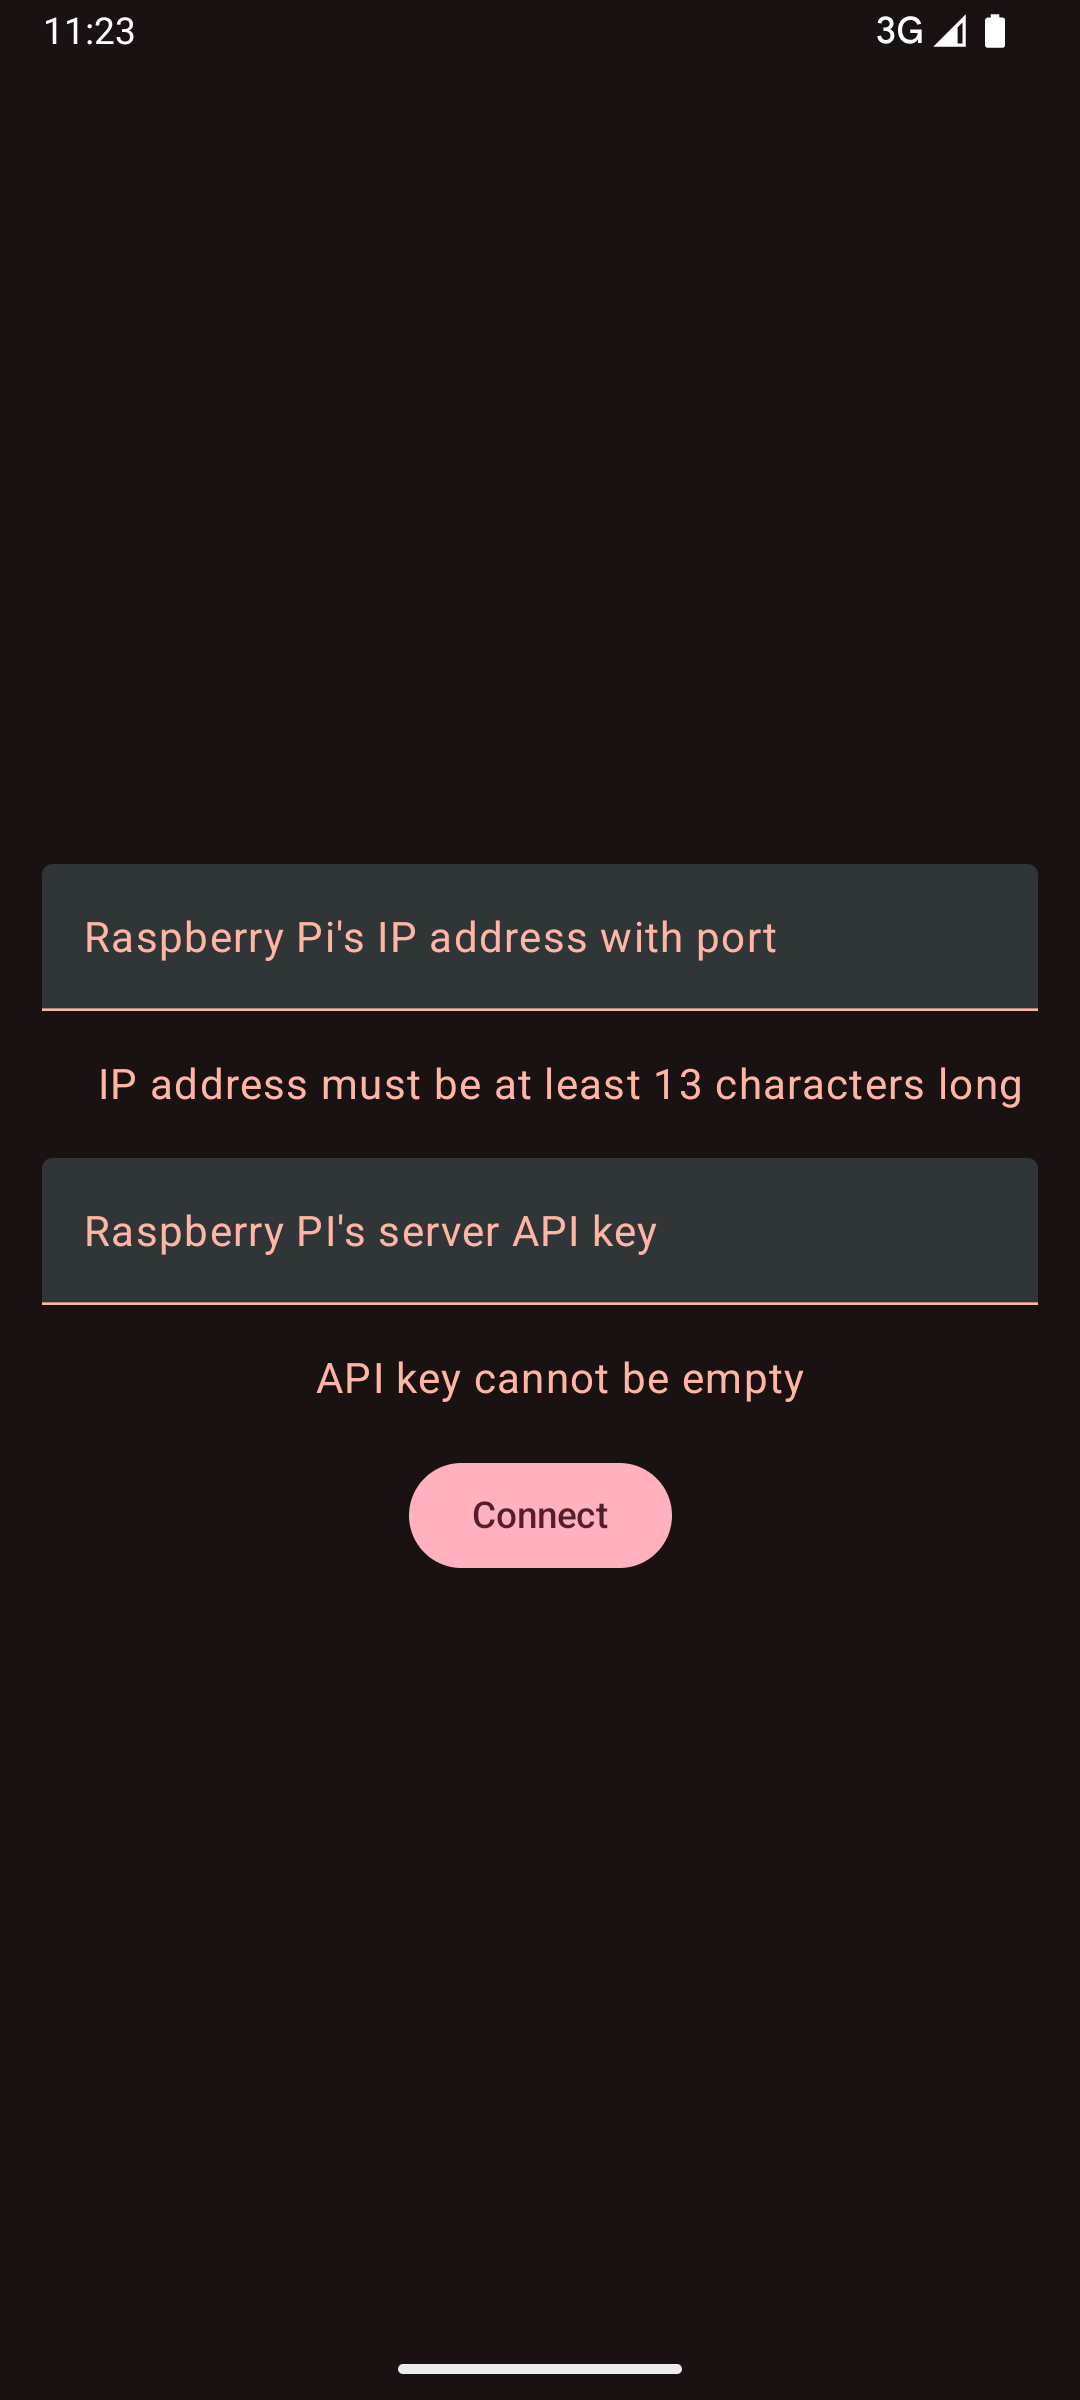
\includegraphics[scale=0.25]{figures/setup_screen_wrong_input.png}
    \caption{Błędne dane w polach tekstowych}
    \label{fig:błędne-dane-setup-screen}
\end{figure}

\clearpage
\noindent Podczas nawiązywania połączenia przycisk zmienia się w animowany wskaźnik postępu, co sygnalizuje użytkownikowi trwającą operację.\\
Ekran \texttt{SetupAndConnect} jest kluczowym elementem aplikacji, ponieważ pozwala na nawiązanie połączenia z serwerem Raspberry Pi, bez którego dalsze funkcjonalności aplikacji nie byłyby
dostępne. Dzięki zastosowaniu walidacji danych oraz przechowywaniu konfiguracji w \textbf{DataStore Preferences}, użytkownik nie musi każdorazowo wprowadzać adresu IP i klucza API, co znacząco
poprawia wygodę korzystania z aplikacji.


\clearpage
\subsubsection{Ekran Home}
Ekran \texttt{Home} pełni rolę głównego widoku aplikacji \texttt{HuePi}, w którym użytkownik może przeglądać listę dostępnych żarówek Philips Hue. Wyświetlane informacje obejmują nazwę żarówki,
jej aktualny kolor, poziom jasności oraz stan (włączona/wyłączona). Użytkownik ma również możliwość odświeżenia listy urządzeń oraz przejścia do ekranu szczegółów konkretnej żarówki.

\begin{figure}[H]
    \centering
    \hypertarget{fig:home-screen}{}
    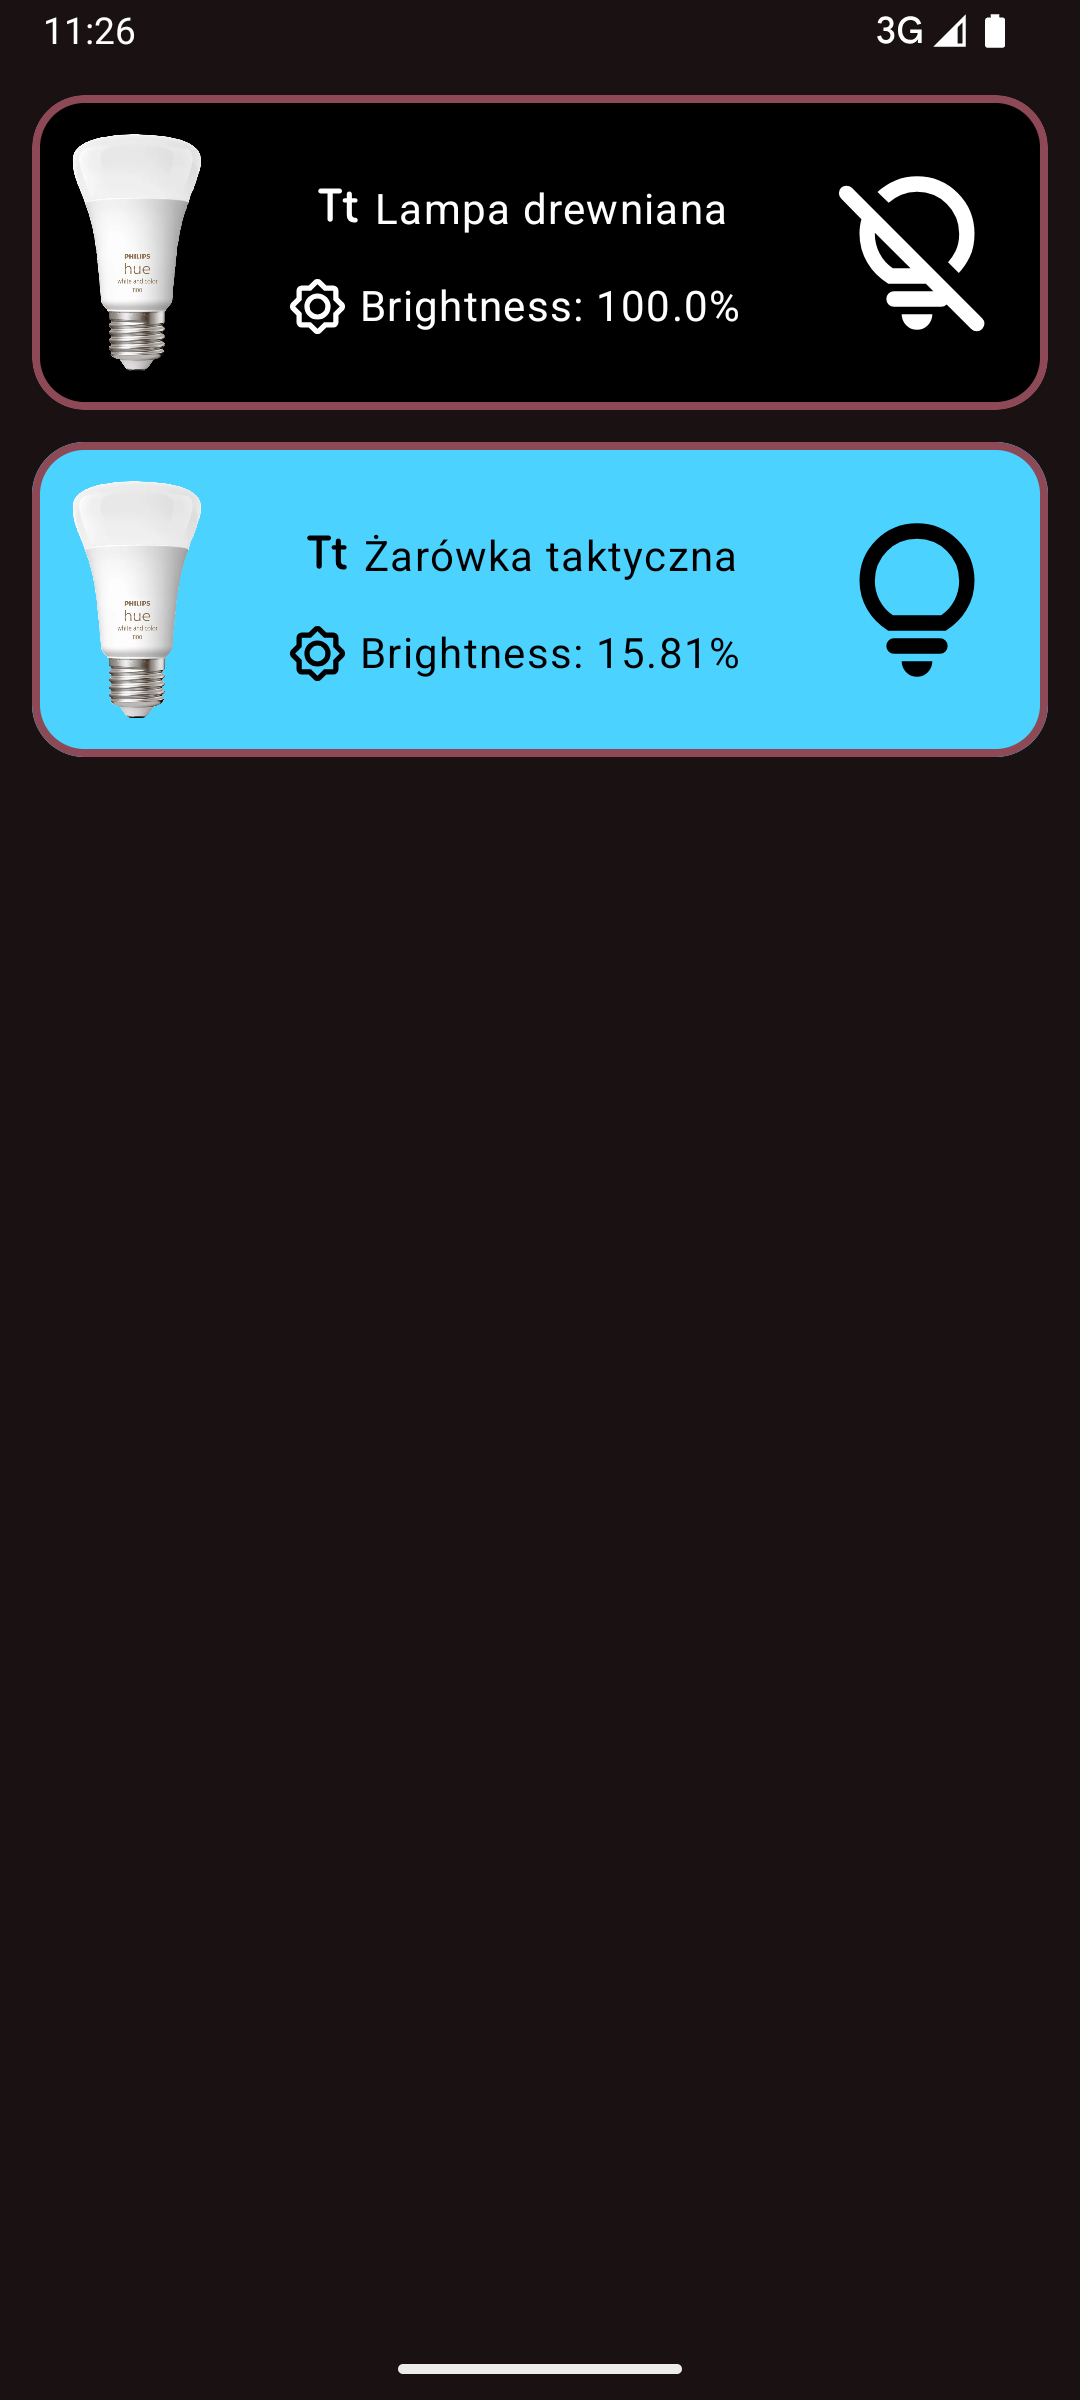
\includegraphics[scale=0.22]{figures/menu_screen.png}
    \caption{Ekran z listą żarówek}
    \label{fig:home-screen}
\end{figure}

\subsubsection*{Struktura plików ekranu}
\noindent Ekran został podzielony na trzy główne pliki:
\begin{itemize}
    \item \textbf{\texttt{HomeScreen.kt}} – główny kontener ekranu, który obsługuje układ interfejsu oraz funkcję \textit{pull-to-refresh}.
    \item \textbf{\texttt{HomeContent.kt}} – definiuje wygląd i zachowanie listy żarówek, obsługuje przypadek, gdy lista jest pusta.
    \item \textbf{\texttt{HomeViewModel.kt}} – zarządza pobieraniem listy żarówek oraz ich stanem, wykorzystując do tego \textbf{Retrofit} i \textbf{DataStore Preferences}.
\end{itemize}

\noindent Podział ten zgodny jest z architekturą \textit{MVVM} (Model-View-ViewModel), dzięki czemu logika biznesowa jest odseparowana od interfejsu użytkownika, co poprawia czytelność kodu
i ułatwia jego testowanie.

\subsubsection*{Interfejs użytkownika}
\noindent Lista żarówek wyświetlana jest w postaci \texttt{LazyColumn}, co pozwala na efektywne renderowanie długich list. Jeśli lista jest pusta, użytkownik widzi komunikat „No light bulbs found!”.
Każdy element listy wyświetlany jest przy użyciu komponentu \texttt{LightBulbItem}, który prezentuje informacje o stanie żarówki.

\begin{lstlisting}[language=Kotlin]
LazyColumn(
    modifier = modifier.fillMaxSize(),
    contentPadding = PaddingValues(12.dp),
    verticalArrangement = Arrangement.spacedBy(12.dp)
) {
    items(lightBulbsList) { lightBulb ->
        LightBulbItem(
            color = Color(lightBulb.color.toColorInt()),
            lightBulbName = lightBulb.name,
            brightnessLevel = lightBulb.brightness,
            lightBulbOn = lightBulb.isOn,
            rid = lightBulb.rid,
            onLightBulbClicked = onLightBulbClicked
        )
    }
}
\end{lstlisting}

\noindent Ekran obsługuje także mechanizm \textit{pull-to-refresh}, który umożliwia użytkownikowi ręczne odświeżenie listy żarówek.

\begin{lstlisting}[language=Kotlin]
PullToRefreshBox(
    state = pullToRefreshState,
    isRefreshing = isRefreshing,
    onRefresh = onRefresh,
    modifier = Modifier.fillMaxSize()
) {
    when {
        isRefreshing -> {}
        lightBulbsList.isNullOrEmpty() -> {
            Box(contentAlignment = Alignment.Center, modifier = Modifier.fillMaxSize()) {
                Text("No light bulbs found!", style = MaterialTheme.typography.bodyLarge)
            }
        }
        else -> {
            HomeContent(
                lightBulbsList = lightBulbsList,
                onLightBulbClicked = onLightBulbClicked,
                modifier = Modifier
                    .statusBarsPadding()
                    .navigationBarsPadding()
            )
        }
    }
}
\end{lstlisting}

\subsubsection*{Pobieranie listy żarówek}
\noindent Dane o żarówkach pobierane są z serwera Raspberry Pi poprzez moduł \textbf{Retrofit}. Plik \texttt{HomeViewModel.kt} zarządza pobieraniem listy świateł i ich przechowywaniem w stanie aplikacji.
Aby uniknąć ponownego wpisywania adresu IP i klucza API, dane te są odczytywane z \textbf{DataStore Preferences}.

\begin{lstlisting}[language=Kotlin]
fun fetchLightBulbs() {
    viewModelScope.launch {
        _isRefreshing.value = true
        try {
            val raspberryIpAddress = dataStoreManager.getRaspberryPiUrl()
            val raspberryApiKey = dataStoreManager.getRaspberryPiApiKey()

            val raspberryPiAPIService = RetrofitInstance.getClient(
                baseUrl = raspberryIpAddress,
                raspberryApiKey = raspberryApiKey
            )

            val lightBulbs = raspberryPiAPIService.getAllLightsDetails().body()
            _lightBulbsList.value = lightBulbs
        } catch (e: Exception) {
            _lightBulbsList.value = null
        } finally {
            _isRefreshing.value = false
        }
    }
}
\end{lstlisting}

\noindent Ekran \texttt{HomeScreen} stanowi główne centrum sterowania dla użytkownika. Pozwala na szybkie przeglądanie aktualnego stanu oświetlenia oraz nawigowanie do ekranu szczegółów konkretnej
żarówki. Dzięki zastosowaniu mechanizmu \textit{pull-to-refresh}, użytkownik ma pełną kontrolę nad aktualizacją wyświetlanych danych.


\subsubsection{Ekran LightDetails}
Ekran \texttt{LightDetailsScreen} umożliwia użytkownikowi sterowanie wybraną żarówką Philips Hue. Po przejściu z ekranu głównego użytkownik ma dostęp do szczegółowych informacji o żarówce oraz
może zmieniać jej stan, jasność, kolor i włączyć tryb dynamicznej zmiany barwy w zależności od temperatury otoczenia.

\subsubsection*{Struktura plików ekranu}
\noindent Ekran został podzielony na trzy pliki:
\begin{itemize}
    \item \textbf{\texttt{LightDetailsScreen.kt}} – główny kontener ekranu, zarządza układem interfejsu i obsługuje mechanizm odświeżania danych.
    \item \textbf{\texttt{LightDetailsContent.kt}} – definiuje widok ekranu, zawierający komponenty do sterowania żarówką (przełącznik zasilania, suwak jasności, wybór koloru).
    \item \textbf{\texttt{LightDetailsViewModel.kt}} – zarządza pobieraniem danych o żarówce oraz obsługą interakcji użytkownika, np. wysyłaniem żądań do serwera Raspberry Pi w celu zmiany ustawień światła.
\end{itemize}

\noindent Podział ten zgodny jest z architekturą \textit{MVVM} (Model-View-ViewModel), co zapewnia oddzielenie logiki biznesowej od warstwy interfejsu użytkownika.

\subsubsection*{Interfejs użytkownika}
\noindent Główne elementy ekranu to:
\begin{itemize}
    \item \textbf{Przełącznik zasilania} – umożliwia włączenie i wyłączenie żarówki.
    \item \textbf{Suwak jasności} – pozwala dostosować poziom jasności światła.
    \item \textbf{Koło wyboru koloru} – umożliwia użytkownikowi zmianę barwy światła przy użyciu selektora kolorów.
    \item \textbf{Tryb zmiany barwy w zależności od temperatury} – opcjonalna funkcja, która pozwala dostosować kolor światła na podstawie danych z czujnika temperatury.
\end{itemize}

\begin{figure}[H]
    \centering
    \hypertarget{fig:light-details-screen}{}
    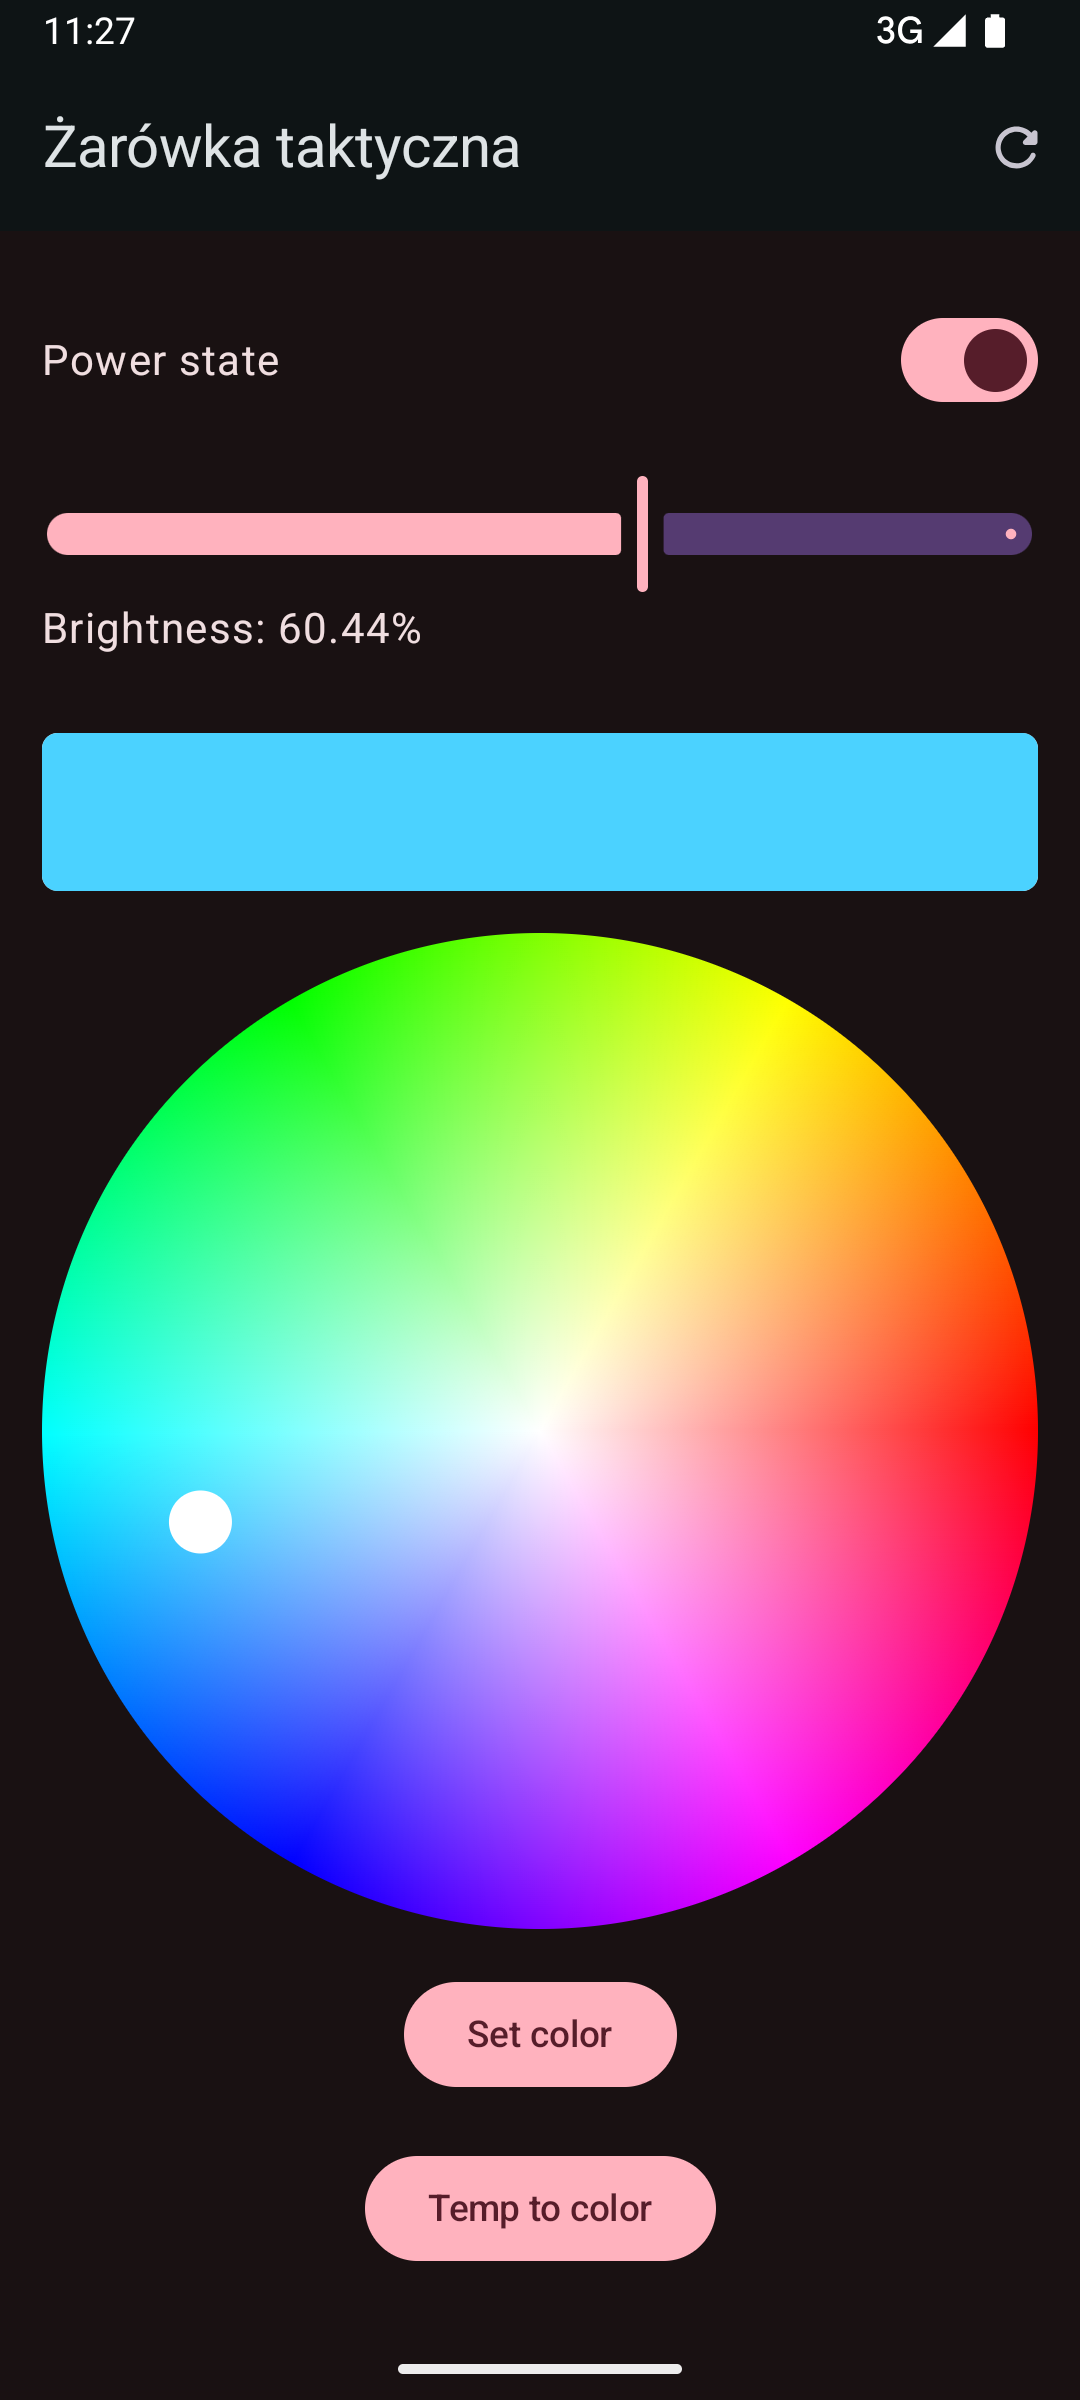
\includegraphics[scale=0.25]{figures/light_detail_screen.png}
    \caption{Ekran ustawień danej żarówki}
    \label{fig:light-details-screen}
\end{figure}

\noindent Dodatkowo użytkownik może odświeżyć dane o żarówce za pomocą ikony odświeżania w górnej części ekranu.

\subsubsection*{Pobieranie danych o żarówce}
\noindent Dane o żarówce są pobierane z serwera Raspberry Pi za pomocą \textbf{Retrofit}. Widok aktualizuje się dynamicznie na podstawie zmian w stanie aplikacji.

\begin{lstlisting}[language=Kotlin]
fun fetchLightBulb() {
    viewModelScope.launch {
        _isFetchingData.value = true
        try {
            raspberryIpAddress = dataStoreManager.getRaspberryPiUrl()
            raspberryApiKey = dataStoreManager.getRaspberryPiApiKey()

            raspberryPiAPIService = RetrofitInstance.getClient(
                baseUrl = raspberryIpAddress,
                raspberryApiKey = raspberryApiKey
            )

            val lightBulb = raspberryPiAPIService.getLightBulbDetails(rid).body()
            _lightBulb.value = lightBulb
        } catch (e: Exception) {
            _lightBulb.value = null
        } finally {
            _isFetchingData.value = false
        }
    }
}
\end{lstlisting}

\subsubsection*{Obsługa zmiany jasności i koloru}
\noindent Użytkownik może dostosować jasność oraz kolor światła za pomocą odpowiednich kontrolek interfejsu. Każda zmiana jest natychmiast wysyłana do serwera.

\begin{lstlisting}[language=Kotlin]
fun changeBrightness(level: Float) {
    viewModelScope.launch {
        val response = raspberryPiAPIService.setBrightness(
            rid = rid,
            level = level
        )
    }
}

fun setColor(h: Float, s: Float, v: Float) {
    viewModelScope.launch {
        val response = raspberryPiAPIService.setColor(
            rid = rid,
            h = h,
            s = s,
            v = v
        )
    }
}
\end{lstlisting}

\subsubsection*{Tryb zmiany barwy w zależności od temperatury}
\noindent Jedną z kluczowych funkcji ekranu \texttt{LightDetailsScreen} jest możliwość aktywowania trybu dynamicznej zmiany barwy światła w zależności od temperatury otoczenia. Funkcja ta została
zaimplementowana w formie \textbf{okna dialogowego}, które pojawia się po naciśnięciu przycisku \texttt{Temp to color}. 

\begin{figure}[H]
    \centering
    \hypertarget{fig:temp-to-color-dialog}{}
    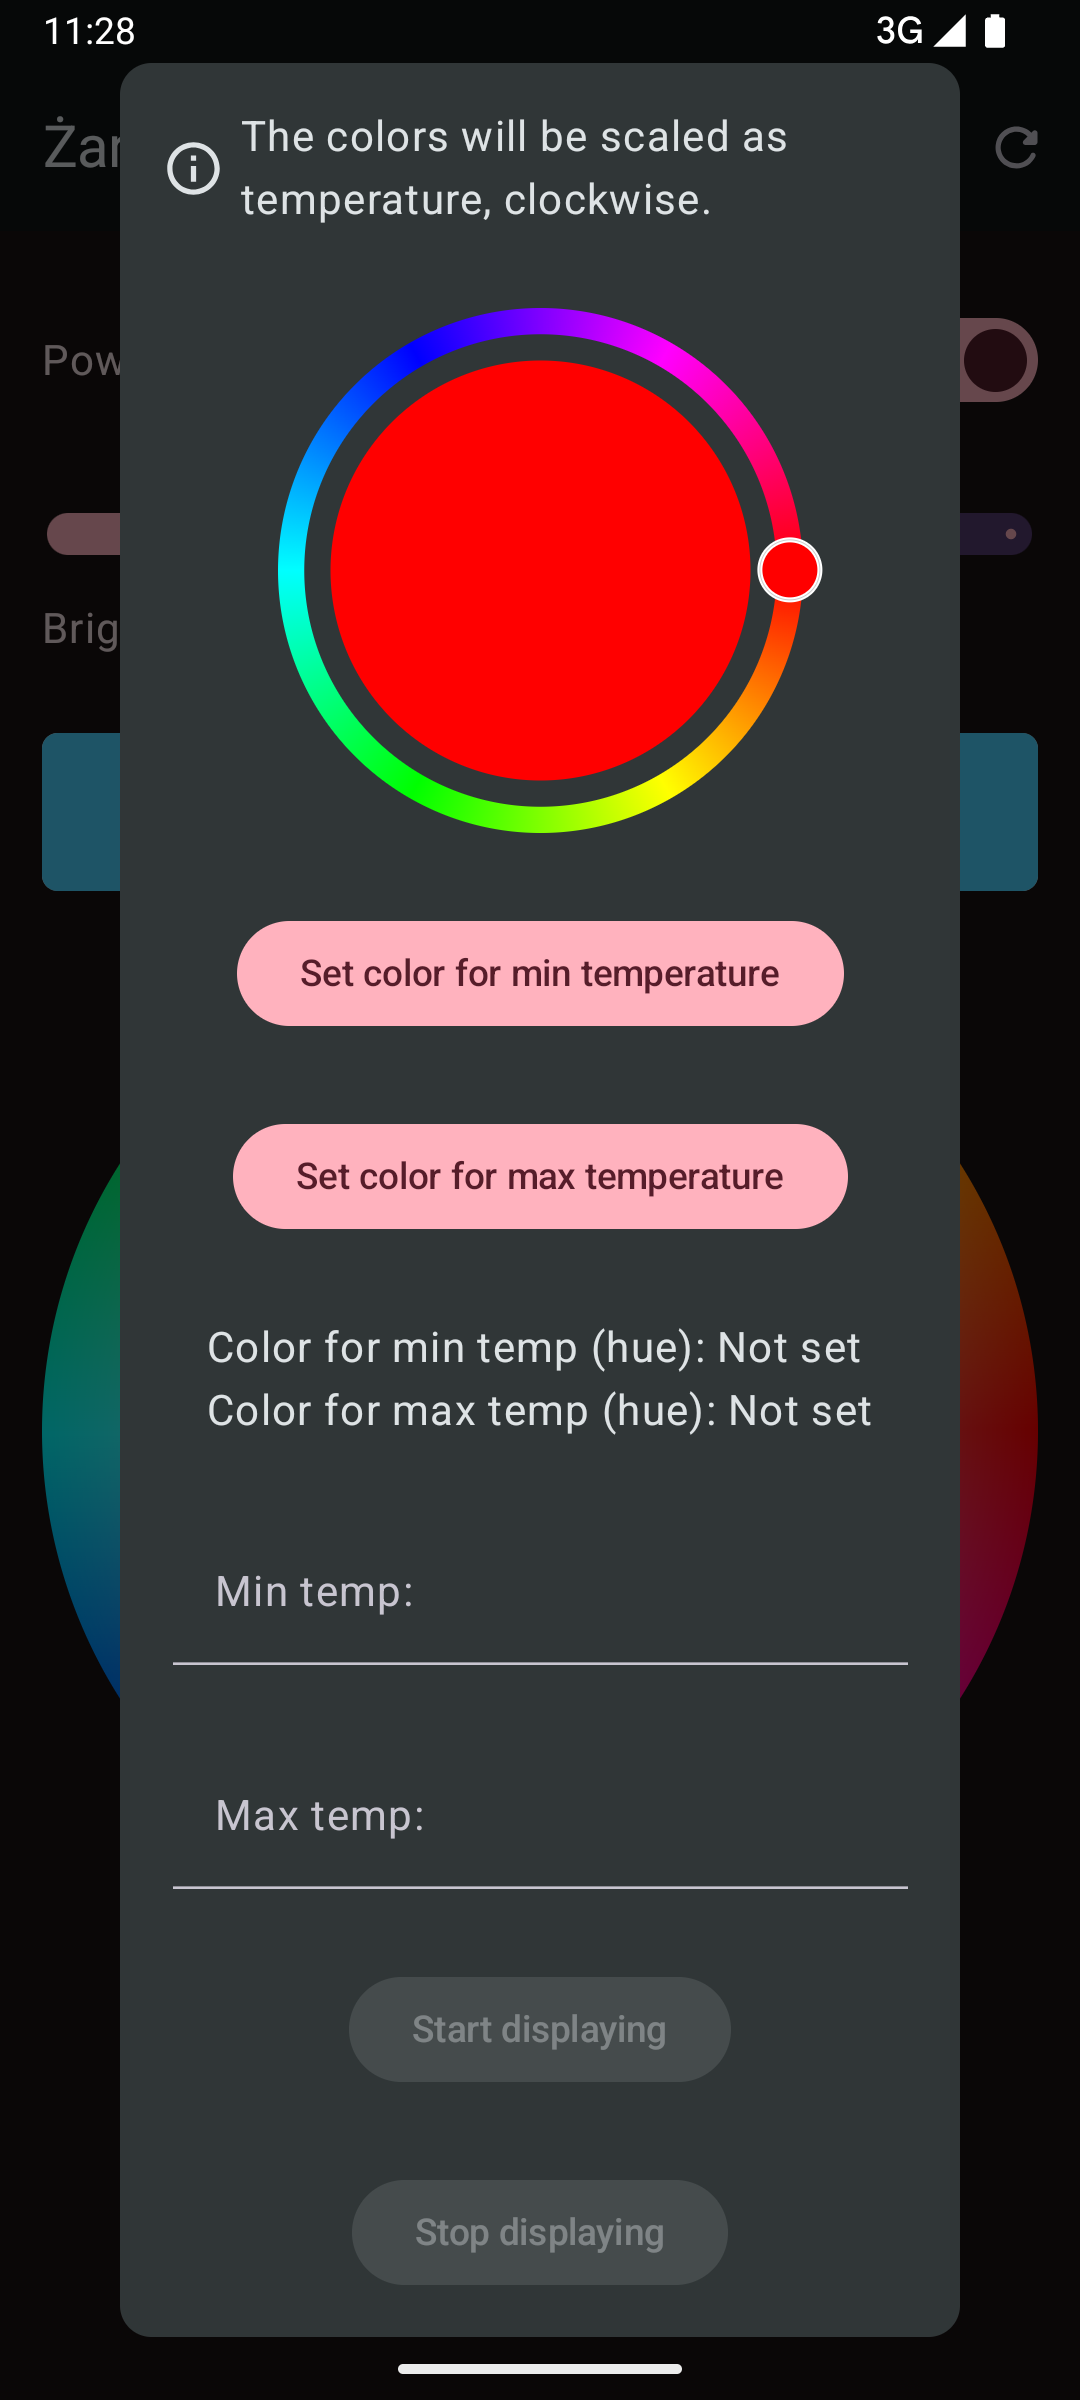
\includegraphics[scale=0.2]{figures/temp_to_color_screen1.png}
    \caption{Okno dialogowe trybu wyświetlania koloru na podstawie temperatury}
    \label{fig:temp-to-color-dialog}
\end{figure}

Po otwarciu okna użytkownik musi ustawić następujące parametry:
\begin{itemize}
    \item \textbf{Minimalna temperatura} – określa najniższą wartość temperatury, przy której światło ma przyjąć wybrany kolor.
    \item \textbf{Maksymalna temperatura} – określa najwyższą wartość temperatury, przy której światło ma przyjąć inny wybrany kolor.
    \item \textbf{Kolor dla minimalnej temperatury} – użytkownik wybiera kolor, który będzie wyświetlany, gdy temperatura osiągnie wartość minimalną.
    \item \textbf{Kolor dla maksymalnej temperatury} – użytkownik wybiera kolor, który będzie wyświetlany, gdy temperatura osiągnie wartość maksymalną.
\end{itemize}

\begin{figure}[H]
    \centering
    \hypertarget{fig:temp-to-color-dialog2}{}
    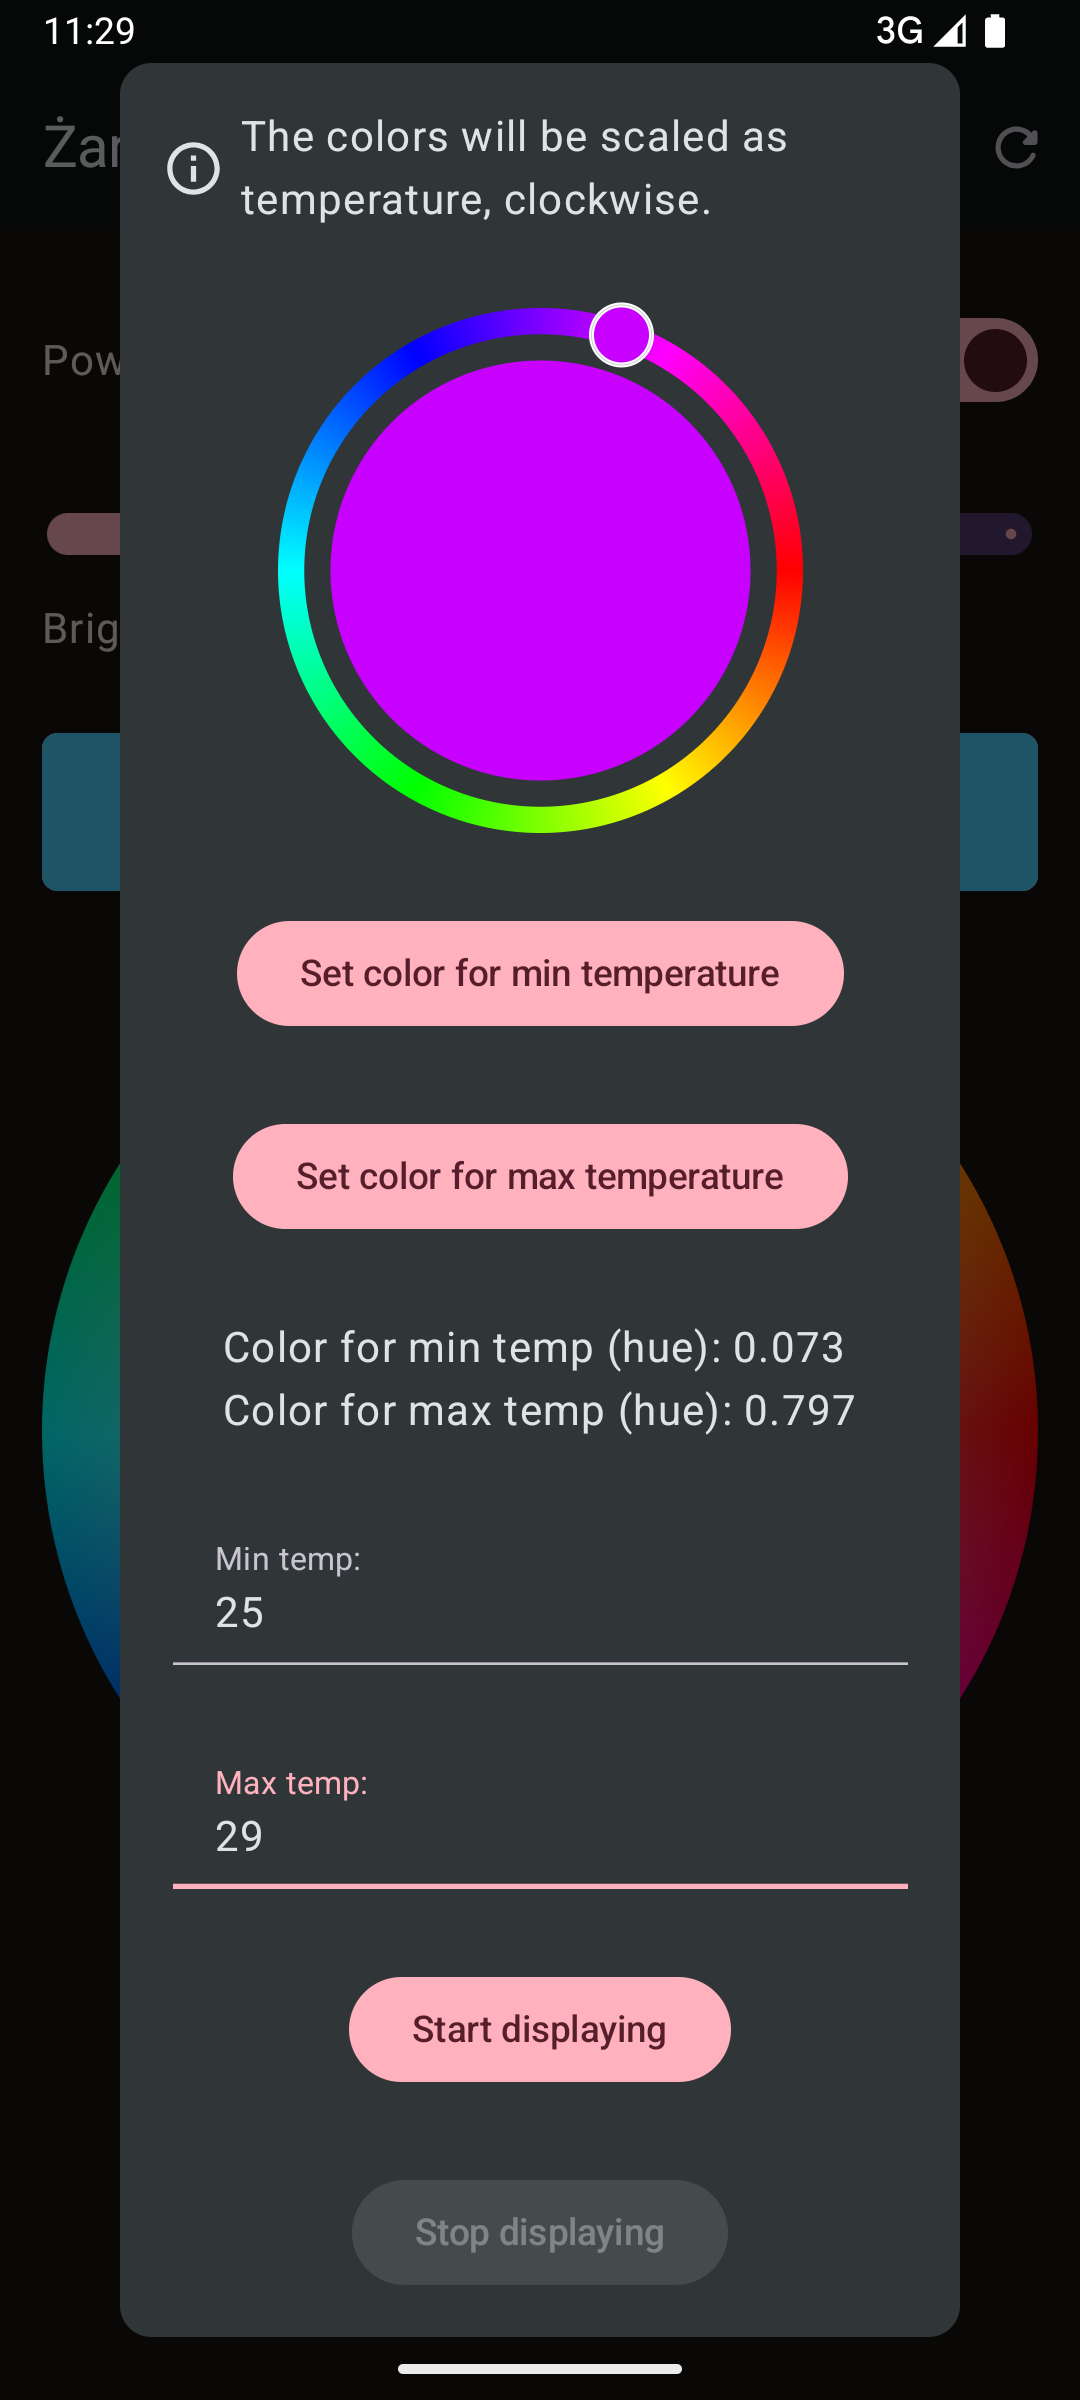
\includegraphics[scale=0.2]{figures/temp_to_color_screen2.png}
    \caption{Okno dialogowe trybu wyświetlania koloru na podstawie temperatury z uzupełnionymi parametrami}
    \label{fig:temp-to-color-dialog2}
\end{figure}

\noindent Aby uprościć konfigurację, użytkownik wybiera kolory na podstawie jednego parametru – wartości \textbf{H (Hue)} z przestrzeni barw \textbf{HSV}. Oznacza to, że nie wybiera on pełnego koloru RGB,
lecz jedynie jego pozycję na palecie barw HSV.

\subsubsection*{Sposób obliczania koloru}
\noindent Gdy funkcja zostanie aktywowana, kolor światła będzie zmieniał się w sposób płynny pomiędzy wartościami wybranymi przez użytkownika. Wartość koloru jest obliczana na podstawie aktualnej
temperatury otoczenia przy użyciu \textbf{interpolacji liniowej} w przestrzeni HSV. Interpolacja odbywa się zgodnie z ruchem wskazówek zegara na palecie HSV. Oznacza to, że jeśli użytkownik wybierze
dla temperatury minimalnej kolor czerwony (\textit{H = 0.0}) i dla temperatury maksymalnej kolor zielony (\textit{H = 0.33}), to w temperaturach pośrednich kolor będzie stopniowo przesuwał się
przez pomarańczowy, żółty aż do zielonego.

\begin{lstlisting}[language=Kotlin]
fun startTempToColorTask(hueMin: Float, hueMax: Float, tempMin: Float, tempMax: Float) {
    viewModelScope.launch {
        val response = raspberryPiAPIService.startTempToColorTask(
            rid = rid,
            hueMin = hueMin,
            hueMax = hueMax,
            tempMin = tempMin,
            tempMax = tempMax
        )
    }
}
\end{lstlisting}

\noindent Wartości te są przesyłane do serwera Raspberry Pi, który na podstawie odczytów z czujnika temperatury oblicza i aktualizuje kolor światła w czasie rzeczywistym.

Tryb dynamicznej zmiany koloru w zależności od temperatury pozwala użytkownikowi na automatyczne dostosowanie oświetlenia do warunków otoczenia. Dzięki intuicyjnemu interfejsowi,
użytkownik może łatwo skonfigurować zakres temperatur i odpowiadające im kolory, co sprawia, że światło zmienia się płynnie zgodnie z ruchem wskazówek zegara na palecie HSV. Jest to
zaawansowana funkcjonalność, która wprowadza dodatkowy poziom automatyzacji w ekosystemie Philips Hue.

\clearpage

\section{Podsumowanie}
Projekt \texttt{HuePi} to kompleksowe rozwiązanie umożliwiające użytkownikowi sterowanie inteligentnym oświetleniem Philips Hue poprzez serwer uruchomiony na \textbf{Raspberry Pi}.
System został zaprojektowany w sposób modularny, wykorzystując nowoczesne technologie zarówno po stronie serwera, jak i aplikacji mobilnej.

\subsection{Główne założenia projektu}
\noindent Głównym celem projektu było stworzenie aplikacji, która pozwala użytkownikowi na wygodne zarządzanie oświetleniem w sposób bardziej elastyczny niż przy użyciu standardowej aplikacji Philips Hue.
Kluczowe założenia obejmowały:
\begin{itemize}
    \item Możliwość sterowania światłami Hue poprzez dedykowany serwer działający na Raspberry Pi.
    \item Rozszerzenie funkcjonalności ekosystemu Hue o obsługę czujnika temperatury BME280.
    \item Intuicyjny interfejs użytkownika, bazujący na \textbf{Jetpack Compose} i wzorcu \textbf{MVVM}.
    \item Implementację dynamicznej zmiany koloru światła w zależności od temperatury otoczenia.
    \item Wsparcie dla pamięci lokalnej (\textbf{DataStore Preferences}), pozwalającej na przechowywanie konfiguracji połączenia.
\end{itemize}

\subsection{Technologie użyte w projekcie}
\noindent W projekcie wykorzystano szereg nowoczesnych technologii, które zapewniają wysoką wydajność i skalowalność systemu:
\begin{itemize}
    \item \textbf{FastAPI} – framework użyty do implementacji serwera REST API na Raspberry Pi.
    \item \textbf{Retrofit} – biblioteka odpowiedzialna za komunikację aplikacji mobilnej z serwerem.
    \item \textbf{Jetpack Compose} – nowoczesny system budowy interfejsu użytkownika w aplikacji mobilnej.
    \item \textbf{DataStore Preferences} – mechanizm zapisywania konfiguracji aplikacji na urządzeniu mobilnym.
    \item \textbf{mDNS} – technologia użyta do automatycznego wykrywania mostka Philips Hue w sieci lokalnej.
\end{itemize}

\subsection{Architektura systemu}
\noindent Projekt został podzielony na dwie główne części:
\begin{itemize}
    \item \textbf{Serwer na Raspberry Pi} – zarządza połączeniem z mostkiem Hue, obsługuje czujnik temperatury i udostępnia API do komunikacji z aplikacją mobilną.
    \item \textbf{Aplikacja mobilna} – pozwala użytkownikowi na sterowanie światłami, przechowuje konfigurację połączenia i dynamicznie pobiera dane z serwera.
\end{itemize}

\noindent Struktura kodu w obu częściach została zaprojektowana zgodnie z dobrymi praktykami programistycznymi, co zapewnia wysoką czytelność i możliwość dalszej rozbudowy systemu.

\subsection{Funkcjonalności aplikacji}
\noindent Aplikacja mobilna dostarcza użytkownikowi bogaty zestaw funkcji:
\begin{itemize}
    \item \textbf{Łączenie z serwerem} – użytkownik może skonfigurować połączenie poprzez podanie adresu IP i klucza API.
    \item \textbf{Lista żarówek} – wyświetlanie wszystkich dostępnych świateł w ekosystemie Hue.
    \item \textbf{Sterowanie żarówką} – możliwość włączania i wyłączania światła, regulacji jasności oraz zmiany koloru.
    \item \textbf{Dynamiczna zmiana koloru} – tryb, w którym kolor światła dostosowuje się do temperatury otoczenia.
    \item \textbf{Odświeżanie danych} – użytkownik może ręcznie aktualizować informacje o dostępnych żarówkach i ich stanie.
\end{itemize}

\subsection{Dalszy rozwój}
\noindent Projekt \texttt{HuePi} udowodnił, że istnieje możliwość rozszerzenia ekosystemu Philips Hue o nowe funkcjonalności, które nie są dostępne w natywnej aplikacji producenta. Dzięki wykorzystaniu
serwera pośredniczącego na Raspberry Pi możliwe jest wprowadzenie niestandardowych funkcji, takich jak zmiana koloru światła w zależności od temperatury. Możliwości dalszego rozwoju projektu obejmują:
\begin{itemize}
    \item Wprowadzenie harmonogramów oświetlenia na podstawie danych z czujników.
    \item Integrację z dodatkowymi urządzeniami z ekosystemu Philips Hue 
    \item Optymalizację komunikacji między aplikacją a serwerem poprzez WebSockety zamiast REST API.
    \item Wsparcie dla sterowania głosowego przy użyciu asystentów, takich jak Google Assistant czy Alexa.
\end{itemize}

\subsection{Wnioski}
Projekt \texttt{HuePi} to nowoczesne rozwiązanie, które łączy elastyczność systemów inteligentnego oświetlenia z możliwościami rozszerzonej automatyki domowej. Dzięki dobrze zaprojektowanej
architekturze, modularności kodu oraz zastosowaniu nowoczesnych technologii, aplikacja zapewnia intuicyjne i wygodne sterowanie oświetleniem Philips Hue. W przyszłości projekt może zostać rozwinięty
o dodatkowe funkcje, co jeszcze bardziej zwiększy jego użyteczność w codziennym użytkowaniu.


\clearpage

\section*{Załączniki}
\addcontentsline{toc}{section}{Załączniki}

Link do repozytorium projektu \url{https://github.com/Klusio19/HuePi}

\clearpage

\addcontentsline{toc}{section}{Literatura}

\begin{thebibliography}{4}
    \bibitem{popularność-smart-home} https://www.statista.com/forecasts/887613/number-of-smart-homes-in-the-smart-home-market-in-the-world
    \bibitem{dokumentacja-philips-hue-app} https://www.philips-hue.com/pl-pl/explore-hue/apps/bridge
    \bibitem{dokumentacja-home-assistant} https://www.home-assistant.io/docs/automation/
    \bibitem{dokumentacja-google-home} https://home.google.com/about-google-home/
    \bibitem{bme280-datasheet} https://www.mouser.com/datasheet/2/783/BST-BME280-DS002-1509607.pdf
    \bibitem{fastapi-automatyczna-dokumentacja} https://fastapi.tiangolo.com/\#interactive-api-docs
    \bibitem{kotlin-data-wydania} https://kotlinlang.org/docs/faq.html
    \bibitem{kotlin-popularność} https://developer.android.com/kotlin
    \bibitem{jetpack-compose-mniej-kodu} https://developer.android.com/develop/ui/compose/why-adopt\#less-code
    \bibitem{retrofit} https://square.github.io/retrofit/

\end{thebibliography}

\clearpage

\makesummary

\end{document}
